\documentclass[11pt,a4paper]{article}

% Image mode: pdf.
% Image paths stay relative. In PDF mode, place same-basename PDF conversions
% of the chapter SVG files in the assets/ directory beside this source.

\usepackage{iftex}
\ifPDFTeX
  \PackageError{handout}{This template requires XeTeX or Tectonic}{Compile with xelatex or tectonic.}
\fi

\usepackage[a4paper,top=18mm,bottom=20mm,left=20mm,right=20mm,headsep=6mm]{geometry}
\usepackage{fontspec}
\usepackage{xeCJK}
\usepackage{amsmath}
\usepackage{unicode-math}

% Font settings are intentionally visible in the generated .tex file.
% These defaults target the macOS machine used for the released PDF.
% Change the family names when compiling on another system.
\setmainfont{Songti TC}
\setsansfont{Heiti TC}
\setmonofont{Menlo}
\setCJKmainfont{Songti TC}
\setCJKsansfont{Heiti TC}
\setCJKmonofont{Heiti TC}
\setmathfont{STIX Two Math}
\XeTeXlinebreaklocale "zh"
\XeTeXlinebreakskip=0pt plus 1pt

\usepackage{xcolor}
\definecolor{HandoutBlue}{HTML}{215A91}
\definecolor{HandoutBlueLight}{HTML}{EEF5FC}
\definecolor{HandoutGreen}{HTML}{39715A}
\definecolor{HandoutGreenLight}{HTML}{EFF8F3}
\definecolor{HandoutGold}{HTML}{8A641C}
\definecolor{HandoutGoldLight}{HTML}{FFF8E8}
\definecolor{HandoutInk}{HTML}{253142}
\definecolor{HandoutMuted}{HTML}{667085}

\usepackage{graphicx}
\makeatletter
% Pandoc 3 emits an accessibility `alt` key for raster/PDF images. Older
% graphicx releases do not know that key, so accept it without changing layout.
\@ifundefined{KV@Gin@alt}{\define@key{Gin}{alt}{}}{}
\newsavebox\pandoc@box
\newcommand*\pandocbounded[1]{%
  \sbox\pandoc@box{#1}%
  \Gscale@div\@tempa{\textheight}{\dimexpr\ht\pandoc@box+\dp\pandoc@box\relax}%
  \Gscale@div\@tempb{\linewidth}{\wd\pandoc@box}%
  \ifdim\@tempb\p@<\@tempa\p@\let\@tempa\@tempb\fi
  \ifdim\@tempa\p@<\p@\scalebox{\@tempa}{\usebox\pandoc@box}%
  \else\usebox{\pandoc@box}%
  \fi
}
\makeatother
\usepackage{float}
\floatplacement{figure}{H}
% Pandoc uses LTcaptype=none for uncaptioned longtables. The caption package
% expects that name to exist as a counter even though it is never displayed.
\newcounter{none}
\usepackage{caption}
\captionsetup[figure]{labelformat=empty,labelsep=none,font=small}

\usepackage{booktabs,longtable,array,calc}
\usepackage{etoolbox}
\makeatletter
\patchcmd\longtable{\par}{\if@noskipsec\mbox{}\fi\par}{}{}
\makeatother

\usepackage[most]{tcolorbox}
\tcbuselibrary{breakable,skins}
\newtcolorbox{HandoutLearningMap}{
  enhanced,breakable,colback=HandoutBlueLight,colframe=HandoutBlue,
  boxrule=0.8pt,arc=1.5mm,left=3mm,right=3mm,top=2mm,bottom=2mm,
  before skip=8pt,after skip=10pt
}
\newtcolorbox{HandoutWorkedExample}{
  enhanced,breakable,colback=HandoutGreenLight,colframe=HandoutGreen,
  boxrule=0.65pt,arc=1.5mm,left=3mm,right=3mm,top=2mm,bottom=2mm,
  before skip=8pt,after skip=10pt
}
\newtcolorbox{HandoutSelfCheck}{
  enhanced,breakable,colback=HandoutGoldLight,colframe=HandoutGold,
  boxrule=0.65pt,arc=1.5mm,left=3mm,right=3mm,top=2mm,bottom=2mm,
  before skip=8pt,after skip=10pt
}

\usepackage{titlesec}
\titleformat{\section}{\sffamily\bfseries\Large\color{HandoutBlue}}{}{0pt}{}
\titleformat{\subsection}{\sffamily\bfseries\large\color{HandoutInk}}{}{0pt}{}
\titleformat{\subsubsection}{\sffamily\bfseries\normalsize\color{HandoutInk}}{}{0pt}{}
\titlespacing*{\section}{0pt}{1.4em}{0.55em}
\titlespacing*{\subsection}{0pt}{1.15em}{0.45em}
\titlespacing*{\subsubsection}{0pt}{0.9em}{0.35em}
\setcounter{secnumdepth}{-\maxdimen}

\usepackage{hyperref}
\usepackage{bookmark}
\IfFileExists{xurl.sty}{\usepackage{xurl}}{}
\urlstyle{same}
\hypersetup{
  colorlinks=true,
  linkcolor=HandoutBlue,
  urlcolor=HandoutBlue,
  citecolor=HandoutBlue,
  pdftitle={數A4-1 空間向量},
  pdfsubject={數學},
  pdfcreator={Pandoc with the HighSchooContent LaTeX template}
}

\setlength{\parindent}{0pt}
\setlength{\parskip}{0.55em plus 0.15em minus 0.1em}
\setlength{\emergencystretch}{3em}
\setlength{\LTpre}{0.5em}
\setlength{\LTpost}{0.5em}
\renewcommand{\arraystretch}{1.18}
\providecommand{\tightlist}{%
  \setlength{\itemsep}{0pt}\setlength{\parskip}{0pt}}
\pagestyle{plain}


\begin{document}

\begin{tcolorbox}[
  enhanced,colback=white,colframe=HandoutBlue,boxrule=1.1pt,arc=2mm,
  borderline west={3pt}{0pt}{HandoutBlue},left=5mm,right=4mm,top=4mm,bottom=4mm
]
{\sffamily\small\bfseries\color{HandoutBlue}學生講義}\par
{\sffamily\bfseries\LARGE\color{HandoutInk}數A4-1 空間向量}\par
\vspace{0.35em}{\large 用三個分量描述空間中的位置、方向、投影、面積與體積}\par
\vspace{0.45em}{\small\color{HandoutMuted}%
科目：數學
\quad 課程：普通高中數學A 第四冊
\quad 版本：學生版｜核心＋理解
\quad 校訂：2026-08-29
}\par
\vspace{0.25em}{\small\color{HandoutMuted}範圍：現行數學A主線；力矩列為外積的直接應用}\par
\end{tcolorbox}


\begin{HandoutLearningMap}

\subsection{本章核心問題}\label{ux672cux7ae0ux6838ux5fc3ux554fux984c}

\begin{enumerate}
\def\labelenumi{\arabic{enumi}.}
\tightlist
\item
  \textbf{空間中的直線與平面有哪些位置關係？}──先判斷是否共平面，再處理平行、相交、垂直與角度。
\item
  \textbf{怎麼把三維位置與方向化成可計算的數字？}──選定三條互相垂直的坐標軸，以三個分量表示點與向量。
\item
  \textbf{怎麼由分量求夾角、垂直與投影？}──內積量出一個方向沿另一方向的有效分量。
\item
  \textbf{怎麼由分量求面積、法向與體積？}──外積建立垂直方向，三重積把底面積與高度合成體積。
\end{enumerate}

{藍色：現行核心}
{青綠：理解支援與用途}
{紫色：由核心直接推出的應用}

\end{HandoutLearningMap}

\section{0. 從平面走進空間}\label{ux5f9eux5e73ux9762ux8d70ux9032ux7a7aux9593}

平面坐標用 \((x,y)\) 表示位置；空間多了一個彼此獨立的方向，因此用 \((x,y,z)\)。這個改變看似只多一個分量，幾何上卻出現一種平面中沒有的關係：兩條直線可以既不相交也不平行，因為它們分處不同平面。

空間向量的主線可整理成四步：

\begin{enumerate}
\def\labelenumi{\arabic{enumi}.}
\tightlist
\item
  先建立點、直線、平面的幾何關係；
\item
  用三個坐標把位置與方向數值化；
\item
  用內積處理角度與投影；
\item
  用外積與三重積處理法向、面積與體積。
\end{enumerate}

工程製圖用三維坐標記錄零件位置；電腦圖學把物體表面化成向量與法向量；機器手臂用內積判斷方向，用外積決定旋轉軸。這些用途都建立在同一套幾何與運算上。

\section{1. 空間中的直線與平面}\label{ux7a7aux9593ux4e2dux7684ux76f4ux7ddaux8207ux5e73ux9762}

\subsection{1.1 基本對象與位置關係}\label{ux57faux672cux5c0dux8c61ux8207ux4f4dux7f6eux95dcux4fc2}

空間中不共線的三點唯一決定一個平面。若直線上的每一點都在平面 \(E\) 上，記為 \(L\subset E\)；若兩平面不重合且有公共點，它們的交集是一條直線。

兩條不同直線在空間中有三種位置關係：

{\def\LTcaptype{none} % do not increment counter
\begin{longtable}[]{@{}lrrl@{}}
\toprule\noalign{}
關係 & 是否共平面 & 交點個數 & 方向關係 \\
\midrule\noalign{}
\endhead
\bottomrule\noalign{}
\endlastfoot
相交 & 是 & \(1\) & 方向不平行 \\
平行 & 是 & \(0\) & 方向平行 \\
歪斜 & 否 & \(0\) & 方向不平行 \\
\end{longtable}
}

\begin{figure}
\centering
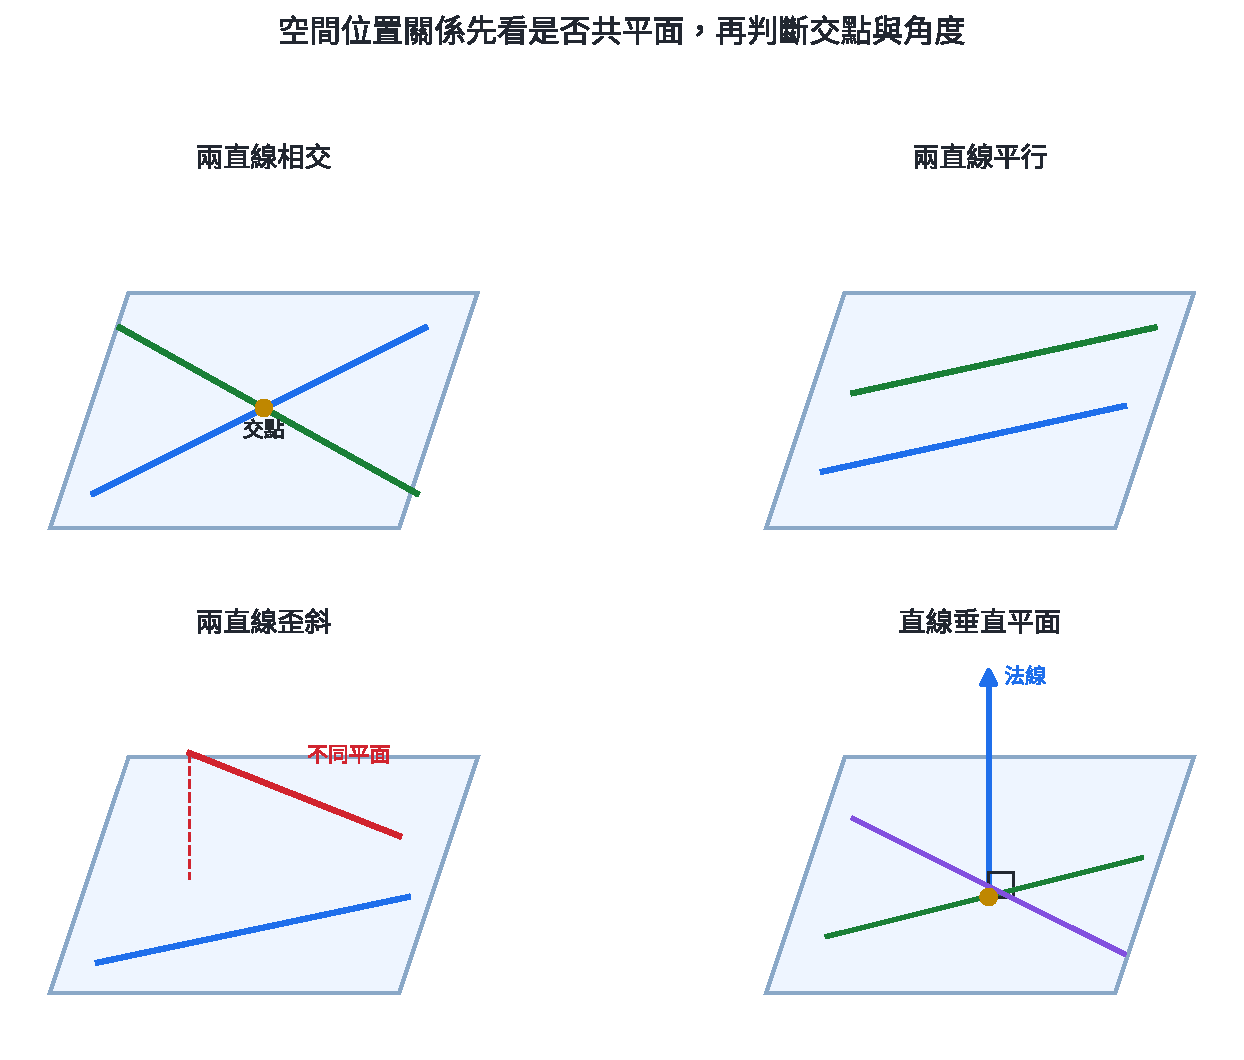
\includegraphics[width=0.96\linewidth,height=\textheight,keepaspectratio,alt={圖 1｜空間位置關係。歪斜線的判斷同時用到「沒有交點」與「不共平面」。}]{assets/數A4-1-直線與平面關係.pdf}
\caption{圖 1｜空間位置關係。歪斜線的判斷同時用到「沒有交點」與「不共平面」。}
\end{figure}

直線與平面的位置關係為：直線在平面上、相交於一點、平行且無交點。兩個不同平面則相交於一直線或互相平行。

空間關係的判斷順序：

\begin{enumerate}
\def\labelenumi{\arabic{enumi}.}
\tightlist
\item
  找出公共點或交集；
\item
  判斷兩對象能否同在一個平面；
\item
  再由方向判斷平行或相交。
\end{enumerate}

「兩直線沒有交點」同時可能對應平行與歪斜；共平面條件把兩者分開。

\subsection{1.2 直線垂直平面}\label{ux76f4ux7ddaux5782ux76f4ux5e73ux9762}

若直線 \(L\) 垂直於平面 \(E\) 內通過交點 \(A\) 的每一條直線，就稱 \(L\) 垂直平面 \(E\)，記為

\[
L\perp E.
\]

實際判定時不必逐一檢查平面內所有直線。平面內兩條相交直線已經給出兩個獨立方向：

設直線 \(m,n\) 在平面 \(E\) 內相交。若

\[
L\perp m,\qquad L\perp n,
\]

而且三線交於同一點，則

\[
\boxed{L\perp E}.
\]

其理由可用向量表達。平面 \(E\) 內通過交點的任一方向都可寫成 \(s\vec m+t\vec n\)。若 \(\vec L\cdot\vec m=0\) 且 \(\vec L\cdot\vec n=0\)，則

\[
\vec L\cdot(s\vec m+t\vec n)
=s(\vec L\cdot\vec m)+t(\vec L\cdot\vec n)=0.
\]

因此 \(L\) 垂直平面內每一個方向。

\subsection{1.3 直線與平面、兩平面的角}\label{ux76f4ux7ddaux8207ux5e73ux9762ux5169ux5e73ux9762ux7684ux89d2}

直線 \(L\) 與平面 \(E\) 相交時，把 \(L\) 正射影到 \(E\) 上。\(L\) 與其投影線的銳角或直角，稱為直線與平面的夾角，範圍為

\[
0^\circ\le\theta\le90^\circ.
\]

若 \(L\perp E\)，夾角為 \(90^\circ\)；若 \(L\parallel E\) 或 \(L\subset E\)，夾角為 \(0^\circ\)。

兩相交平面的交線為 \(g\)。在兩平面內分別取垂直 \(g\) 的直線 \(m,n\)，\(m,n\) 的夾角稱為兩平面的夾角。由兩個半平面形成的角稱為二面角；指定內部區域後，角度可以介於 \(0^\circ\) 與 \(180^\circ\)。

\subsection{1.4 三垂線定理}\label{ux4e09ux5782ux7ddaux5b9aux7406}

設 \(P\) 在平面 \(E\) 外，\(PA\perp E\)，\(B\) 在平面 \(E\) 上。線段 \(AB\) 是斜線 \(PB\) 在平面上的正射影。若平面內直線 \(L\) 通過 \(B\) 且 \(L\perp AB\)，則

\[
\boxed{L\perp PB}.
\]

\begin{figure}
\centering
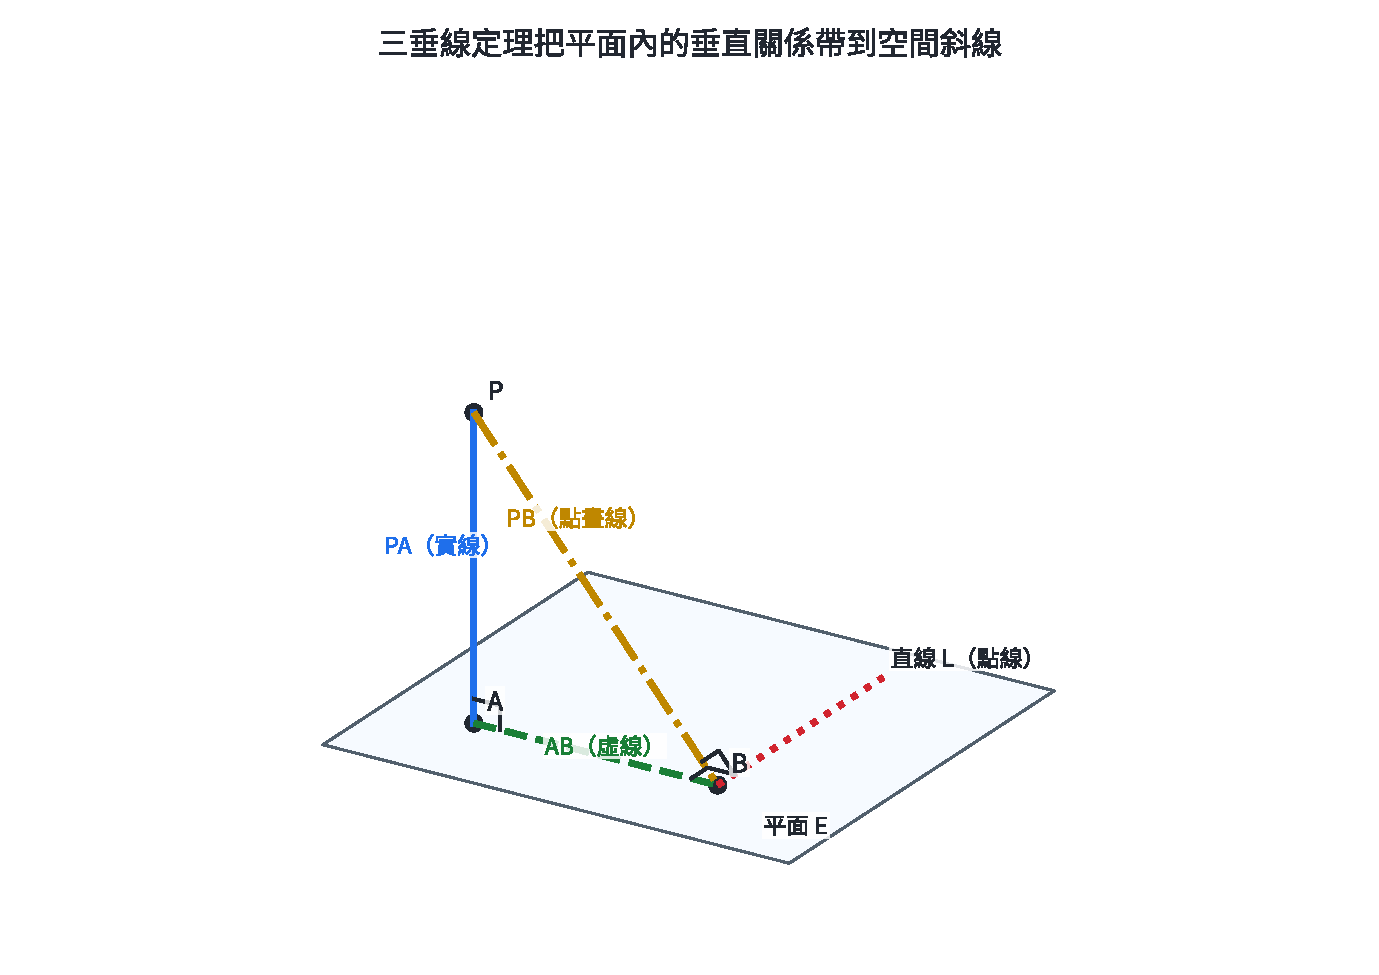
\includegraphics[width=0.82\linewidth,height=\textheight,keepaspectratio,alt={圖 2｜三垂線定理。PA 垂直平面，AB 是 PB 的投影；L\textbackslash perp AB 會推出 L\textbackslash perp PB。}]{assets/數A4-1-三垂線定理.pdf}
\caption{圖 2｜三垂線定理。\(PA\) 垂直平面，\(AB\) 是 \(PB\) 的投影；\(L\perp AB\) 會推出 \(L\perp PB\)。}
\end{figure}

把 \(\overrightarrow{BP}\) 分解成平面內與平面外的部分：

\[
\overrightarrow{BP}=\overrightarrow{BA}+\overrightarrow{AP}.
\]

\(L\perp AB\) 給出 \(\vec L\cdot\overrightarrow{BA}=0\)；\(PA\perp E\) 給出 \(\vec L\cdot\overrightarrow{AP}=0\)。所以

\[
\vec L\cdot\overrightarrow{BP}=0+0=0,
\]

也就是 \(L\perp PB\)。定理的核心是：斜線分成「平面內投影」與「垂直平面的高度」，一條平面內直線若同時垂直這兩部分，也垂直它們的合向量。

\begin{HandoutWorkedExample}

\subsection{完整示範｜判斷兩條不相交直線}\label{ux5b8cux6574ux793aux7bc4ux5224ux65b7ux5169ux689dux4e0dux76f8ux4ea4ux76f4ux7dda}

長方體 \(ABCD-EFGH\) 中，\(E,F,G,H\) 分別在 \(A,B,C,D\) 正上方。判斷 \(AB\) 與 \(CG\)、\(AB\) 與 \(HG\) 的位置關係。

\textbf{\(AB\) 與 \(CG\)：} \(AB\) 是底面水平邊，\(CG\) 是鉛直邊；兩線沒有交點，方向也不平行。若它們共平面，該平面同時包含 \(B,C\) 方向的底面位移與 \(CG\) 的鉛直方向，並會包含通過 \(B\) 的鉛直線 \(BF\)；但 \(AB\) 的另一端 \(A\) 不在側面 \(BCGF\)。因此兩線歪斜。

\textbf{\(AB\) 與 \(HG\)：} 在長方體中，對應邊方向相同，而且可共同放在斜截面 \(ABGH\) 中，所以

\[
AB\parallel HG.
\]

沒有交點只完成第一步；共平面與方向共同決定結論。

\end{HandoutWorkedExample}

\begin{HandoutWorkedExample}

\subsection{完整示範｜由投影三角形求直線與平面的角}\label{ux5b8cux6574ux793aux7bc4ux7531ux6295ux5f71ux4e09ux89d2ux5f62ux6c42ux76f4ux7ddaux8207ux5e73ux9762ux7684ux89d2}

點 \(P\) 到平面 \(E\) 的垂足為 \(A\)，\(B\) 在平面上。已知 \(PA=6\)、\(AB=8\)，求斜線 \(PB\) 與平面 \(E\) 的夾角。

因 \(PA\perp E\)，所以 \(PA\perp AB\)，三角形 \(PAB\) 在 \(A\) 為直角。\(PB\) 在平面上的投影是 \(AB\)。設所求角為 \(\theta=\angle PBA\)，則

\[
PB=\sqrt{6^2+8^2}=10,
\]

\[
\sin\theta=\frac{PA}{PB}=\frac{6}{10}=\frac35,
\qquad
\tan\theta=\frac{PA}{AB}=\frac{6}{8}=\frac34.
\]

因此

\[
\boxed{\theta=\sin^{-1}\!\left(\frac35\right)\approx36.9^\circ}.
\]

高度越大、水平投影越短，斜線與平面的夾角越大。

\end{HandoutWorkedExample}

\begin{HandoutWorkedExample}

\subsection{完整示範｜用三垂線定理建立空間垂直}\label{ux5b8cux6574ux793aux7bc4ux7528ux4e09ux5782ux7ddaux5b9aux7406ux5efaux7acbux7a7aux9593ux5782ux76f4}

在圖 2 的設定中，\(PA\perp E\)，\(AB\perp L\)，且 \(A,B,L\) 都在平面 \(E\) 內。證明 \(PB\perp L\)。

由 \(PA\perp E\)，可知 \(PA\) 垂直平面內的 \(L\)。題設又給 \(AB\perp L\)。因此 \(L\) 同時垂直 \(\overrightarrow{BA}\) 與 \(\overrightarrow{AP}\)。由

\[
\overrightarrow{BP}=\overrightarrow{BA}+\overrightarrow{AP},
\]

得到

\[
\vec L\cdot\overrightarrow{BP}
=\vec L\cdot\overrightarrow{BA}+\vec L\cdot\overrightarrow{AP}=0.
\]

故 \(PB\perp L\)。

\end{HandoutWorkedExample}

\begin{HandoutSelfCheck}

\subsection{節末練習｜空間位置與角度}\label{ux7bc0ux672bux7df4ux7fd2ux7a7aux9593ux4f4dux7f6eux8207ux89d2ux5ea6}

\begin{enumerate}
\def\labelenumi{\arabic{enumi}.}
\tightlist
\item
  兩條不同直線 \(L_1,L_2\) 都平行同一平面 \(E\)。列出 \(L_1,L_2\) 可能的位置關係。
\item
  正方體 \(ABCD-EFGH\) 中，列出一條與 \(AC\) 歪斜的棱。
\item
  點 \(P\) 到平面 \(E\) 的距離為 \(5\)，斜線 \(PB\) 長 \(13\)。求 \(PB\) 在 \(E\) 上的投影長及 \(PB\) 與 \(E\) 的夾角。
\item
  平面 \(E\) 內兩相交直線 \(m,n\) 交於 \(A\)。直線 \(L\) 通過 \(A\)，且 \(L\perp m\)、\(L\perp n\)。說明 \(L\) 與 \(E\) 的關係。
\item
  \(PA\perp E\)，\(A,B,C\) 在 \(E\) 上，且 \(AB\perp BC\)。證明 \(PB\perp BC\)。
\item
  兩平面交於直線 \(g\)。在兩平面內分別取 \(m\perp g\)、\(n\perp g\)，且 \(m,n\) 交於同一點。若 \(\angle(m,n)=68^\circ\)，求兩平面的銳二面角。
\end{enumerate}

\textbf{解答}

\begin{enumerate}
\def\labelenumi{\arabic{enumi}.}
\tightlist
\item
  可能相交、平行或歪斜。各直線平行 \(E\) 只限制它們不穿過 \(E\)；兩線彼此是否共平面仍有三種可能。
\item
  例如 \(BF\)。\(AC\) 在底面，\(BF\) 為鉛直棱，兩線無交點、方向不平行且不共平面，所以歪斜。
\item
  投影長設為 \(x\)。由直角三角形，\(x=\sqrt{13^2-5^2}=12\)。若夾角為 \(\theta\)，\(\sin\theta=5/13\)，所以 \(\theta\approx22.6^\circ\)。
\item
  平面內相交的 \(m,n\) 給出兩個獨立方向；\(L\) 同時垂直兩方向，故 \(L\perp E\)。
\item
  \(AB\) 是 \(PB\) 在 \(E\) 上的投影；\(BC\perp AB\)，由三垂線定理得 \(PB\perp BC\)。
\item
  兩平面夾角由各平面內垂直交線的兩線夾角定義，因此銳二面角為 \(68^\circ\)。
\end{enumerate}

\end{HandoutSelfCheck}

\section{2. 空間坐標與向量運算}\label{ux7a7aux9593ux5750ux6a19ux8207ux5411ux91cfux904bux7b97}

\subsection{2.1 右手坐標系、坐標平面與投影}\label{ux53f3ux624bux5750ux6a19ux7cfbux5750ux6a19ux5e73ux9762ux8207ux6295ux5f71}

取共同交於原點 \(O\)、兩兩垂直的 \(x,y,z\) 軸。正向依右手規則排列：右手四指由 \(x\) 軸正向轉向 \(y\) 軸正向時，大拇指指向 \(z\) 軸正向。

三個坐標平面為

\[
xy\text{ 平面}:z=0,\qquad
yz\text{ 平面}:x=0,\qquad
zx\text{ 平面}:y=0.
\]

點 \(P=(a,b,c)\) 在三個坐標平面上的正射影分別為

\[
(a,b,0),\qquad(0,b,c),\qquad(a,0,c).
\]

\begin{figure}
\centering
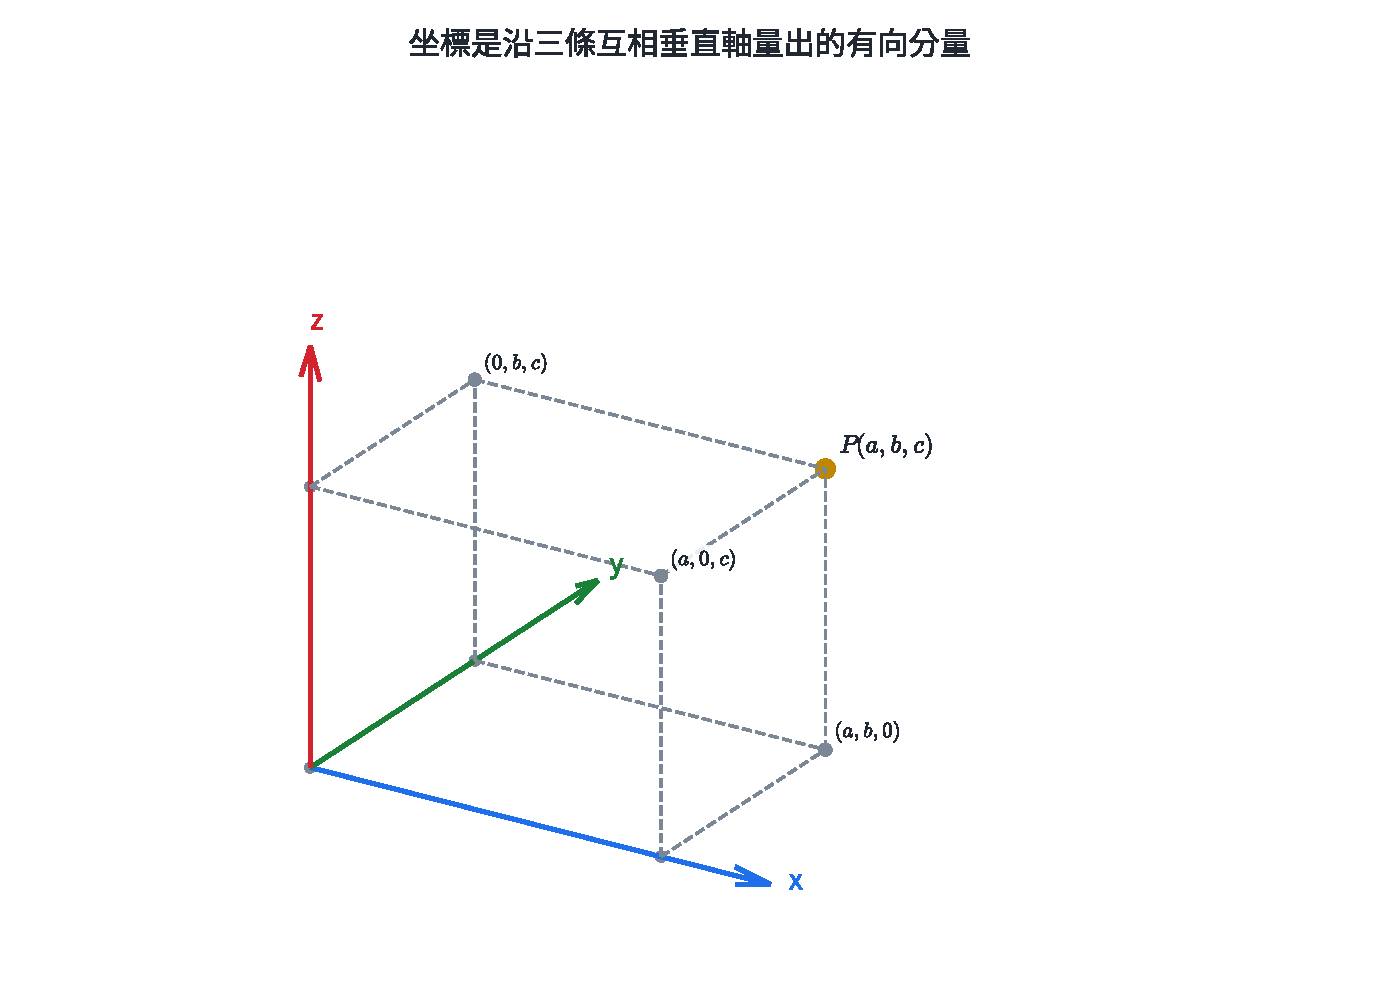
\includegraphics[width=0.82\linewidth,height=\textheight,keepaspectratio,alt={圖 3｜點 P(a,b,c) 的三個分量與在坐標平面上的投影。}]{assets/數A4-1-空間坐標與投影.pdf}
\caption{圖 3｜點 \(P(a,b,c)\) 的三個分量與在坐標平面上的投影。}
\end{figure}

點到三個坐標平面的距離分別是 \(|c|,|a|,|b|\)；點到三條坐標軸的距離則保留垂直於該軸的兩個分量。例如

\[
d(P,x\text{ 軸})=\sqrt{b^2+c^2}.
\]

\subsection{2.2 距離、中點與分點}\label{ux8dddux96e2ux4e2dux9edeux8207ux5206ux9ede}

設 \(A=(x_1,y_1,z_1)\)、\(B=(x_2,y_2,z_2)\)。由三個互相垂直方向依序套用畢氏定理：

\[
\boxed{
AB=\sqrt{(x_2-x_1)^2+(y_2-y_1)^2+(z_2-z_1)^2}
}.
\]

中點為

\[
\boxed{
M=\left(\frac{x_1+x_2}{2},\frac{y_1+y_2}{2},\frac{z_1+z_2}{2}\right)
}.
\]

若 \(P\) 內分 \(AB\) 且 \(AP:PB=m:n\)，則

\[
\boxed{P=\frac{nA+mB}{m+n}}.
\]

權重與相鄰線段交叉配對：\(P\) 靠近哪個端點，那個端點的權重就較大。例如 \(m<n\) 表示 \(AP<PB\)，公式中 \(A\) 的權重 \(n\) 大於 \(B\) 的權重 \(m\)，所以 \(P\) 靠近 \(A\)。

\begin{figure}
\centering
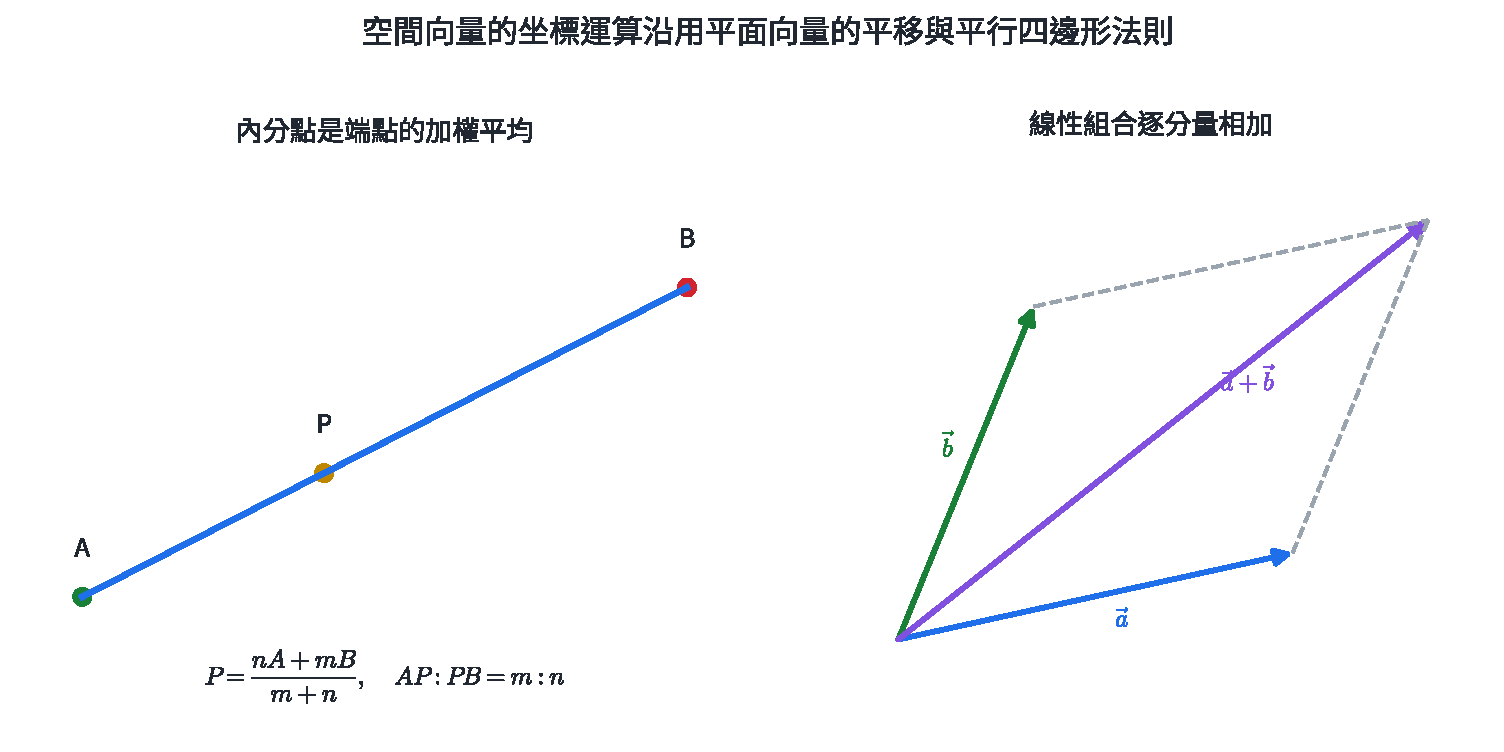
\includegraphics[width=0.96\linewidth,height=\textheight,keepaspectratio,alt={圖 4｜左：內分點是端點的加權平均；右：向量加法逐分量進行。}]{assets/數A4-1-向量坐標與分點.pdf}
\caption{圖 4｜左：內分點是端點的加權平均；右：向量加法逐分量進行。}
\end{figure}

\subsection{2.3 空間向量的坐標與運算}\label{ux7a7aux9593ux5411ux91cfux7684ux5750ux6a19ux8207ux904bux7b97}

設 \(A=(x_1,y_1,z_1)\)、\(B=(x_2,y_2,z_2)\)，則

\[
\boxed{
\overrightarrow{AB}=(x_2-x_1,y_2-y_1,z_2-z_1)
}.
\]

若 \(\vec a=(a_1,a_2,a_3)\)、\(\vec b=(b_1,b_2,b_3)\)，則

\[
\vec a+\vec b=(a_1+b_1,a_2+b_2,a_3+b_3),
\]

\[
k\vec a=(ka_1,ka_2,ka_3),
\]

\[
\boxed{|\vec a|=\sqrt{a_1^2+a_2^2+a_3^2}}.
\]

這些公式源自坐標軸方向的獨立性：同一方向的位移互相累加，三個方向分別處理。

\subsection{2.4 平行、單位向量與線性組合}\label{ux5e73ux884cux55aeux4f4dux5411ux91cfux8207ux7ddaux6027ux7d44ux5408}

對非零向量 \(\vec a\)，同方向單位向量為

\[
\boxed{\hat a=\frac{\vec a}{|\vec a|}}.
\]

兩個非零向量平行的條件為

\[
\boxed{\vec a\parallel\vec b\iff\vec b=k\vec a}
\]

其中 \(k>0\) 表示同方向，\(k<0\) 表示反方向。

若 \(\vec a,\vec b,\vec c\) 不共面，空間中每一向量 \(\vec v\) 都能唯一寫成

\[
\boxed{\vec v=x\vec a+y\vec b+z\vec c}.
\]

三個不共面的方向能生成整個空間；係數 \((x,y,z)\) 就是相對於這組基底的坐標。若三向量共面，它們的線性組合仍停留在同一平面，無法生成平面外的方向。

\subsection{坐標分量把幾何轉成可操作資料}\label{ux5750ux6a19ux5206ux91cfux628aux5e7eux4f55ux8f49ux6210ux53efux64cdux4f5cux8cc7ux6599}

工程圖上的每個孔位由三個坐標指定；機器手臂末端的位移由三個分量相加；遊戲引擎把角色位置、速度與攝影機方向都儲存成三維向量。

分量表示保留了幾何的核心：點相減得到位移、向量相加得到合位移、倍數關係判斷平行。只要坐標軸與單位固定，同一套運算可直接交給測量儀器與電腦執行。

\begin{HandoutWorkedExample}

\subsection{完整示範｜投影、距離與對稱點}\label{ux5b8cux6574ux793aux7bc4ux6295ux5f71ux8dddux96e2ux8207ux5c0dux7a31ux9ede}

設 \(P=(3,-4,12)\)。

\begin{enumerate}
\def\labelenumi{\arabic{enumi}.}
\item
  在 \(xy\) 平面上的投影為 \(P_{xy}=(3,-4,0)\)。
\item
  到 \(z\) 軸的距離只看 \(x,y\) 分量：

  \[
  d(P,z\text{ 軸})=\sqrt{3^2+(-4)^2}=5.
  \]
\item
  關於 \(xy\) 平面的對稱點保留 \(x,y\)，反轉垂直於平面的 \(z\) 分量，因此為

  \[
  P'=(3,-4,-12).
  \]
\item
  到原點距離為

  \[
  OP=\sqrt{3^2+(-4)^2+12^2}=13.
  \]
\end{enumerate}

投影、距離與鏡射都可由「哪些分量沿著目標平面、哪些分量垂直目標平面」直接判斷。

\end{HandoutWorkedExample}

\begin{HandoutWorkedExample}

\subsection{完整示範｜內分點與路徑比例}\label{ux5b8cux6574ux793aux7bc4ux5167ux5206ux9edeux8207ux8defux5f91ux6bd4ux4f8b}

無人機由 \(A=(1,2,0)\) 直線飛向 \(B=(11,-3,5)\)。飛完總路程的 \(40\%\) 時位於 \(P\)，求 \(P\)。

因 \(AP:PB=2:3\)，可用分點公式：

\[
P=\frac{3A+2B}{5}
=\frac{3(1,2,0)+2(11,-3,5)}5
=(5,0,2).
\]

也可用參數式核對：

\[
P=A+0.4(B-A)
=(1,2,0)+0.4(10,-5,5)
=(5,0,2).
\]

\(P-A=(4,-2,2)\) 正好是 \(B-A=(10,-5,5)\) 的 \(0.4\) 倍，比例與方向一致。

\end{HandoutWorkedExample}

\begin{HandoutWorkedExample}

\subsection{完整示範｜用線性組合還原三維位移}\label{ux5b8cux6574ux793aux7bc4ux7528ux7ddaux6027ux7d44ux5408ux9084ux539fux4e09ux7dadux4f4dux79fb}

設

\[
\vec a=(1,1,0),\qquad
\vec b=(0,1,1),\qquad
\vec c=(1,0,1).
\]

求 \(x,y,z\) 使

\[
x\vec a+y\vec b+z\vec c=(5,4,3).
\]

比較三個分量：

\[
\begin{cases}
x+z=5,\\
x+y=4,\\
y+z=3.
\end{cases}
\]

前兩式相加再減第三式，得 \(2x=6\)，所以 \(x=3\)。接著 \(y=1\)、\(z=2\)。因此

\[
\boxed{(5,4,3)=3\vec a+\vec b+2\vec c}.
\]

代回三個分量可同時驗證結果。

\end{HandoutWorkedExample}

\begin{HandoutSelfCheck}

\subsection{節末練習｜坐標與向量運算}\label{ux7bc0ux672bux7df4ux7fd2ux5750ux6a19ux8207ux5411ux91cfux904bux7b97}

\begin{enumerate}
\def\labelenumi{\arabic{enumi}.}
\tightlist
\item
  點 \(P=(-2,3,6)\) 在 \(yz\) 平面、\(zx\) 平面上的投影各為何？求 \(P\) 到 \(x\) 軸的距離。
\item
  \(A=(1,-2,3)\)、\(B=(5,4,-1)\)。求 \(\overrightarrow{AB}\)、\(AB\) 與中點 \(M\)。
\item
  \(P\) 內分 \(A=(-1,2,4)\)、\(B=(9,-3,-1)\)，且 \(AP:PB=3:2\)。求 \(P\)。
\item
  已知 \(\vec a=(2,-1,2)\)。求與 \(\vec a\) 同方向的單位向量，以及長度為 \(12\)、方向相反的向量。
\item
  判斷 \(\vec a=(2,-4,6)\) 與 \(\vec b=(-1,2,-3)\) 是否平行，並說明方向。
\item
  設 \(\vec a=(1,0,1)\)、\(\vec b=(0,1,1)\)、\(\vec c=(1,1,0)\)。求 \(x,y,z\) 使 \(x\vec a+y\vec b+z\vec c=(4,5,3)\)。
\end{enumerate}

\textbf{解答}

\begin{enumerate}
\def\labelenumi{\arabic{enumi}.}
\tightlist
\item
  投影分別為 \((0,3,6)\)、\((-2,0,6)\)。到 \(x\) 軸距離為 \(\sqrt{3^2+6^2}=3\sqrt5\)。
\item
  \(\overrightarrow{AB}=(4,6,-4)\)，所以 \(AB=\sqrt{16+36+16}=2\sqrt{17}\)；\(M=(3,1,1)\)。
\item
  \(P=(2A+3B)/5=(5,-1,1)\)。核對 \(P-A=(6,-3,-3)\)、\(B-P=(4,-2,-2)\)，長度比為 \(3:2\)。
\item
  \(|\vec a|=3\)，同方向單位向量為 \((2/3,-1/3,2/3)\)。方向相反且長 \(12\) 的向量為 \(-4\vec a=(-8,4,-8)\)。
\item
  \(\vec b=-\tfrac12\vec a\)，所以平行且方向相反。
\item
  比較分量得 \(x+z=4\)、\(y+z=5\)、\(x+y=3\)。解得 \(x=1\)、\(y=2\)、\(z=3\)。
\end{enumerate}

\end{HandoutSelfCheck}

\section{3. 空間向量的內積、夾角與投影}\label{ux7a7aux9593ux5411ux91cfux7684ux5167ux7a4dux593eux89d2ux8207ux6295ux5f71}

\subsection{3.1 內積的幾何定義與坐標公式}\label{ux5167ux7a4dux7684ux5e7eux4f55ux5b9aux7fa9ux8207ux5750ux6a19ux516cux5f0f}

設 \(\vec a,\vec b\) 為非零向量，夾角 \(\theta\) 取在 \(0\le\theta\le\pi\)。內積定義為

\[
\boxed{
\vec a\cdot\vec b=|\vec a|\,|\vec b|\cos\theta
}.
\]

若其中一向量為零向量，定義內積為 \(0\)。

在直角坐標系中，令

\[
\vec a=(a_1,a_2,a_3),\qquad
\vec b=(b_1,b_2,b_3),
\]

則

\[
\boxed{
\vec a\cdot\vec b=a_1b_1+a_2b_2+a_3b_3
}.
\]

坐標公式可由三個單位基向量 \(\vec i,\vec j,\vec k\) 推出。因三軸兩兩垂直，

\[
\vec i\cdot\vec i=
\vec j\cdot\vec j=
\vec k\cdot\vec k=1,
\]

\[
\vec i\cdot\vec j=
\vec j\cdot\vec k=
\vec k\cdot\vec i=0.
\]

把 \(\vec a=a_1\vec i+a_2\vec j+a_3\vec k\)、\(\vec b=b_1\vec i+b_2\vec j+b_3\vec k\) 展開，交叉方向的乘積全為 \(0\)，只留下同方向的三項。

\begin{figure}
\centering
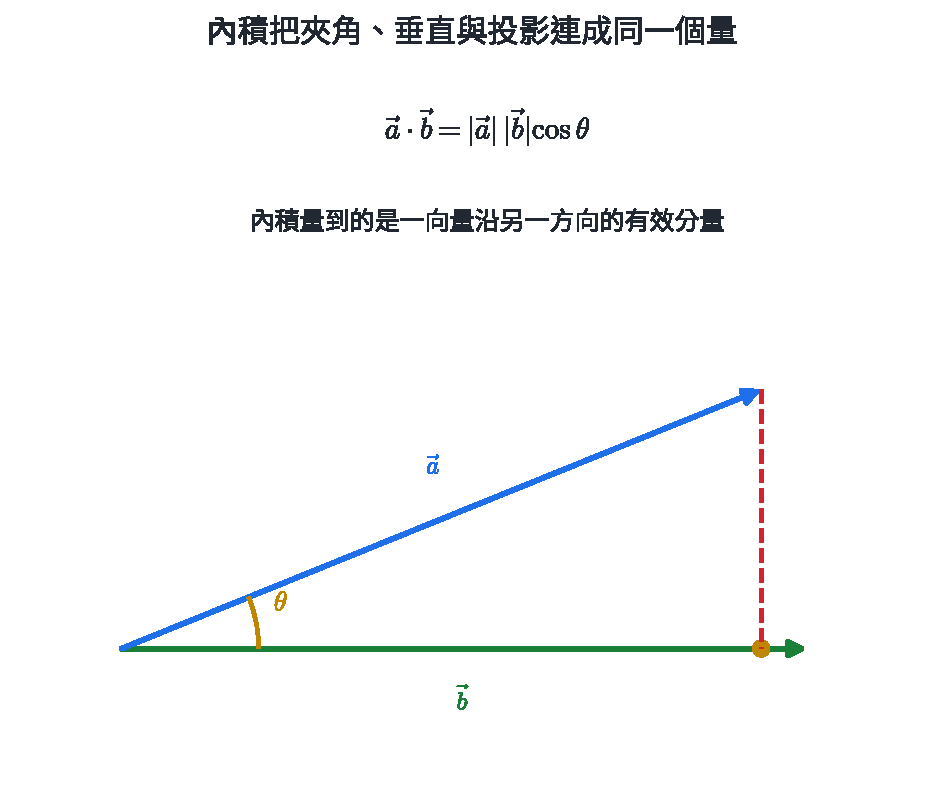
\includegraphics[width=0.86\linewidth,height=\textheight,keepaspectratio,alt={圖 5｜內積等於一向量的長度乘上另一向量沿該方向的帶號投影。}]{assets/數A4-1-內積與夾角.pdf}
\caption{圖 5｜內積等於一向量的長度乘上另一向量沿該方向的帶號投影。}
\end{figure}

內積正負直接描述方向：

{\def\LTcaptype{none} % do not increment counter
\begin{longtable}[]{@{}rrl@{}}
\toprule\noalign{}
\(\vec a\cdot\vec b\) & \(\cos\theta\) & 夾角 \\
\midrule\noalign{}
\endhead
\bottomrule\noalign{}
\endlastfoot
\(>0\) & \(>0\) & 銳角 \\
\(=0\) & \(=0\) & 直角 \\
\(<0\) & \(<0\) & 鈍角 \\
\end{longtable}
}

對非零向量，垂直條件為

\[
\boxed{\vec a\perp\vec b\iff\vec a\cdot\vec b=0}.
\]

夾角可由

\[
\boxed{
\cos\theta=
\frac{\vec a\cdot\vec b}{|\vec a|\,|\vec b|}
}
\]

求得。分母要求兩向量皆非零。

\subsection{3.2 內積的運算性質}\label{ux5167ux7a4dux7684ux904bux7b97ux6027ux8cea}

內積滿足

\[
\vec a\cdot\vec b=\vec b\cdot\vec a,
\]

\[
(s\vec a+t\vec b)\cdot\vec c
=s(\vec a\cdot\vec c)+t(\vec b\cdot\vec c),
\]

\[
\vec a\cdot\vec a=|\vec a|^2.
\]

因此向量和、差的長度可直接展開：

\[
|\vec a+\vec b|^2
=|\vec a|^2+2\vec a\cdot\vec b+|\vec b|^2,
\]

\[
|\vec a-\vec b|^2
=|\vec a|^2-2\vec a\cdot\vec b+|\vec b|^2.
\]

這就是餘弦定理的向量版本。若 \(\vec a\perp\vec b\)，中間項為 \(0\)，公式化成畢氏定理。

\subsection{3.3 正射影與垂直分解}\label{ux6b63ux5c04ux5f71ux8207ux5782ux76f4ux5206ux89e3}

要找 \(\vec a\) 沿 \(\vec b\) 的部分，先取 \(\vec b\) 的單位方向 \(\hat b=\vec b/|\vec b|\)。帶號投影長為

\[
\boxed{
\operatorname{comp}_{\vec b}\vec a
=\vec a\cdot\hat b
=\frac{\vec a\cdot\vec b}{|\vec b|}
}.
\]

投影向量再乘回單位方向：

\[
\boxed{
\operatorname{proj}_{\vec b}\vec a
=\frac{\vec a\cdot\vec b}{|\vec b|^2}\vec b
}.
\]

剩餘部分

\[
\vec a_\perp
=\vec a-\operatorname{proj}_{\vec b}\vec a
\]

會與 \(\vec b\) 垂直，因為

\[
\vec a_\perp\cdot\vec b
=\vec a\cdot\vec b
-\frac{\vec a\cdot\vec b}{|\vec b|^2}(\vec b\cdot\vec b)=0.
\]

\begin{figure}
\centering
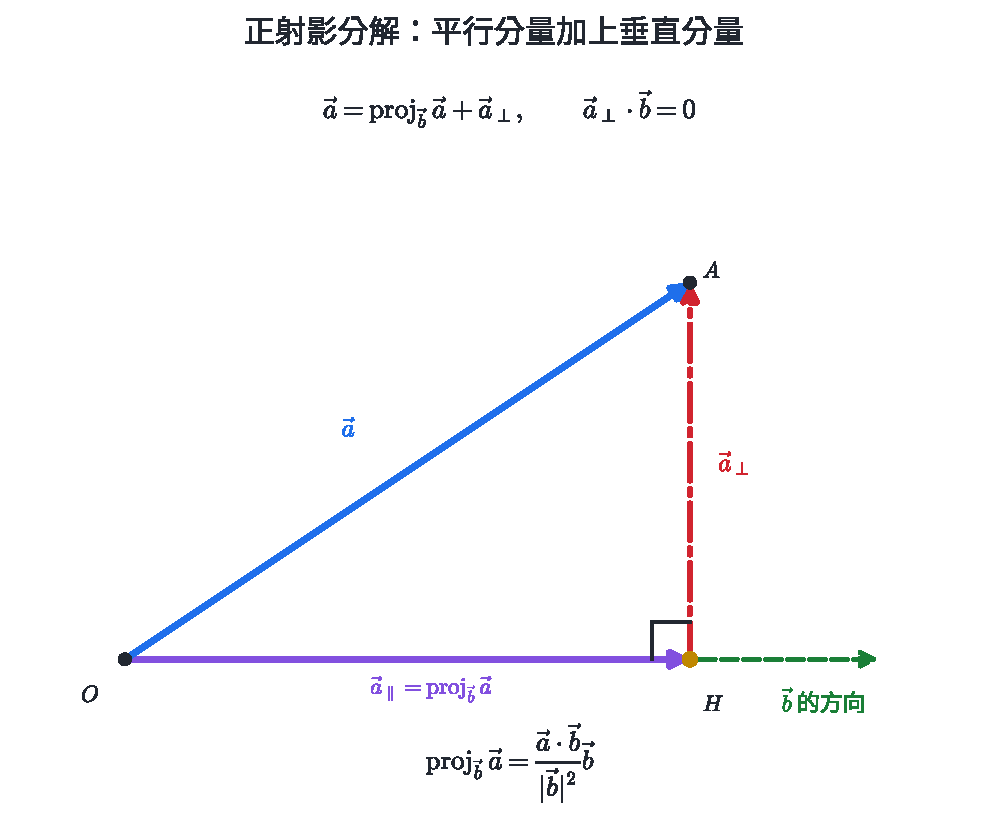
\includegraphics[width=0.88\linewidth,height=\textheight,keepaspectratio,alt={圖 6｜\textbackslash vec a 分成平行於 \textbackslash vec b 的投影與垂直於 \textbackslash vec b 的剩餘分量。}]{assets/數A4-1-正射影分解.pdf}
\caption{圖 6｜\(\vec a\) 分成平行於 \(\vec b\) 的投影與垂直於 \(\vec b\) 的剩餘分量。}
\end{figure}

這個分解直接給出點到直線的距離。直線通過 \(A\)、方向向量為 \(\vec d\)，點 \(P\) 到直線的位移為 \(\overrightarrow{AP}\)。扣掉沿直線方向的投影後，剩下的垂直分量長度就是最短距離：

\[
\boxed{
d(P,L)=
\left|
\overrightarrow{AP}
-\frac{\overrightarrow{AP}\cdot\vec d}{|\vec d|^2}\vec d
\right|}.
\]

垂足 \(H\) 則是

\[
\boxed{
H=A+\frac{\overrightarrow{AP}\cdot\vec d}{|\vec d|^2}\vec d
}.
\]

\subsection{3.4 柯西不等式與等號條件}\label{ux67efux897fux4e0dux7b49ux5f0fux8207ux7b49ux865fux689dux4ef6}

投影向量的長度最多等於原向量長度：

\[
\left|
\operatorname{proj}_{\vec b}\vec a
\right|
=\frac{|\vec a\cdot\vec b|}{|\vec b|}
\le |\vec a|.
\]

兩邊乘以 \(|\vec b|\)，得到柯西不等式：

\[
\boxed{
|\vec a\cdot\vec b|
\le|\vec a|\,|\vec b|
}.
\]

坐標形式為

\[
\boxed{
(a_1b_1+a_2b_2+a_3b_3)^2
\le
(a_1^2+a_2^2+a_3^2)(b_1^2+b_2^2+b_3^2)
}.
\]

等號成立於其中一向量為零，或兩個非零向量平行。

\begin{figure}
\centering
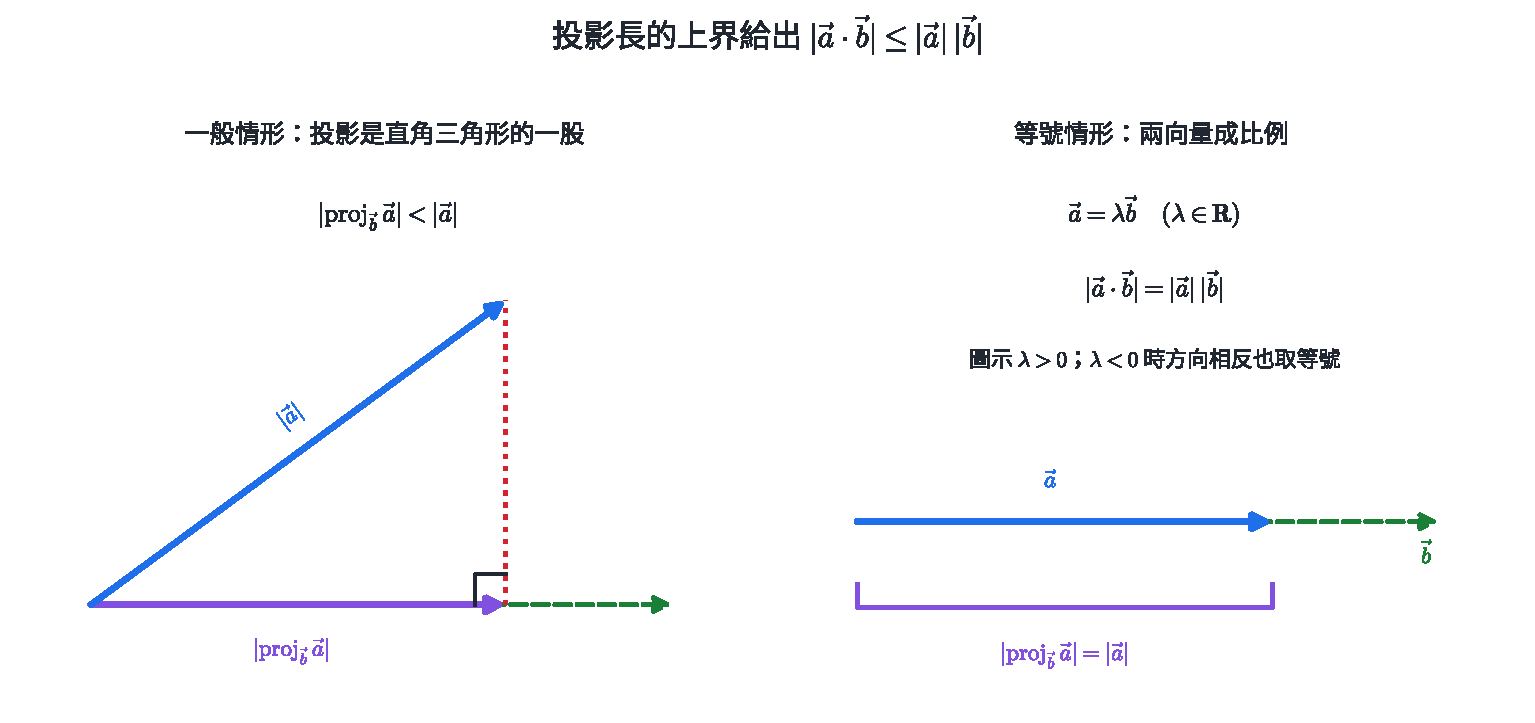
\includegraphics[width=0.95\linewidth,height=\textheight,keepaspectratio,alt={圖 7｜一般情形的投影短於原向量；兩向量成比例時，投影長等於原向量長，柯西不等式取等號。}]{assets/數A4-1-柯西不等式幾何.pdf}
\caption{圖 7｜一般情形的投影短於原向量；兩向量成比例時，投影長等於原向量長，柯西不等式取等號。}
\end{figure}

柯西不等式常把一次式的極值轉成向量長度。若 \(x^2+y^2+z^2=r^2\)，則

\[
|ax+by+cz|
\le\sqrt{a^2+b^2+c^2}\,r.
\]

等號位置與 \((x,y,z)\) 平行於 \((a,b,c)\)，因此不只給極值，也給出達到極值的點。

\subsection{投影保留對指定方向真正有效的部分}\label{ux6295ux5f71ux4fddux7559ux5c0dux6307ux5b9aux65b9ux5411ux771fux6b63ux6709ux6548ux7684ux90e8ux5206}

太陽能板接收的光通量取決於光線沿板面法向的分量；一個力對某方向做功，取決於力沿位移方向的分量；電腦圖學判斷表面亮暗，也要比較光線與表面法向的內積。

內積把「方向有多一致」化成一個數。正值代表大致同向，零代表互不貢獻，負值代表反向。投影再把這個數還原成沿指定方向的向量。

\begin{HandoutWorkedExample}

\subsection{完整示範｜由內積求夾角與垂直參數}\label{ux5b8cux6574ux793aux7bc4ux7531ux5167ux7a4dux6c42ux593eux89d2ux8207ux5782ux76f4ux53c3ux6578}

設

\[
\vec a=(1,2,2),\qquad
\vec b=(2,1,-2).
\]

先算

\[
\vec a\cdot\vec b=2+2-4=0,
\]

所以 \(\vec a\perp\vec b\)，夾角為 \(90^\circ\)。

若改成 \(\vec c=(k,1,-1)\)，要求 \(\vec a\perp\vec c\)，則

\[
\vec a\cdot\vec c=k+2-2=k.
\]

垂直條件給 \(k=0\)。此時 \(\vec c=(0,1,-1)\)，代回內積確為 \(0\)。

\end{HandoutWorkedExample}

\begin{HandoutWorkedExample}

\subsection{完整示範｜求正射影、垂直分量與垂足}\label{ux5b8cux6574ux793aux7bc4ux6c42ux6b63ux5c04ux5f71ux5782ux76f4ux5206ux91cfux8207ux5782ux8db3}

設 \(\vec a=(3,4,1)\)、\(\vec b=(2,1,2)\)。先算

\[
\vec a\cdot\vec b=6+4+2=12,
\qquad
|\vec b|^2=4+1+4=9.
\]

因此

\[
\operatorname{proj}_{\vec b}\vec a
=\frac{12}{9}\vec b
=\left(\frac83,\frac43,\frac83\right).
\]

垂直分量為

\[
\vec a_\perp
=(3,4,1)-\left(\frac83,\frac43,\frac83\right)
=\left(\frac13,\frac83,-\frac53\right).
\]

核對垂直性：

\[
\vec a_\perp\cdot\vec b
=\frac23+\frac83-\frac{10}3=0.
\]

若直線從原點沿 \(\vec b\) 前進，點 \(A=(3,4,1)\) 在直線上的垂足就是

\[
H=\left(\frac83,\frac43,\frac83\right),
\]

點線距離為

\[
|\vec a_\perp|
=\frac13\sqrt{1+64+25}=\sqrt{10}.
\]

\end{HandoutWorkedExample}

\begin{HandoutWorkedExample}

\subsection{完整示範｜由兩點與方向求點線距離}\label{ux5b8cux6574ux793aux7bc4ux7531ux5169ux9edeux8207ux65b9ux5411ux6c42ux9edeux7ddaux8dddux96e2}

直線 \(L\) 通過 \(A=(1,0,2)\)，方向向量 \(\vec d=(2,1,2)\)；點 \(P=(4,4,1)\)。求 \(P\) 到 \(L\) 的垂足與距離。

先取

\[
\overrightarrow{AP}=(3,4,-1).
\]

沿直線方向的參數為

\[
t=\frac{\overrightarrow{AP}\cdot\vec d}{|\vec d|^2}
=\frac{6+4-2}{4+1+4}
=\frac89.
\]

所以垂足

\[
H=A+t\vec d
=\left(\frac{25}{9},\frac89,\frac{34}{9}\right).
\]

垂直位移為

\[
\overrightarrow{HP}
=P-H
=\left(\frac{11}{9},\frac{28}{9},-\frac{25}{9}\right).
\]

它與 \(\vec d\) 的內積為 \((22+28-50)/9=0\)，所以確實垂直。距離為

\[
d(P,L)=|\overrightarrow{HP}|
=\frac{\sqrt{121+784+625}}9
=\frac{\sqrt{1530}}9
=\frac{\sqrt{170}}3.
\]

\end{HandoutWorkedExample}

\begin{HandoutWorkedExample}

\subsection{完整示範｜柯西不等式求球面上的線性式極值}\label{ux5b8cux6574ux793aux7bc4ux67efux897fux4e0dux7b49ux5f0fux6c42ux7403ux9762ux4e0aux7684ux7ddaux6027ux5f0fux6975ux503c}

已知 \(x^2+y^2+z^2=9\)，求 \(2x-y+2z\) 的最大值與最小值，並找出等號位置。

把 \((x,y,z)\) 與係數向量 \((2,-1,2)\) 做內積：

\[
|2x-y+2z|
\le
\sqrt{x^2+y^2+z^2}\sqrt{2^2+(-1)^2+2^2}
=3\cdot3=9.
\]

所以範圍為

\[
\boxed{-9\le2x-y+2z\le9}.
\]

最大值要求 \((x,y,z)\) 與 \((2,-1,2)\) 同方向，且長度為 \(3\)。係數向量本身長度也是 \(3\)，所以最大值在

\[
(x,y,z)=(2,-1,2)
\]

取得；最小值在反方向 \((-2,1,-2)\) 取得。

\end{HandoutWorkedExample}

\begin{HandoutSelfCheck}

\subsection{節末練習｜內積與投影}\label{ux7bc0ux672bux7df4ux7fd2ux5167ux7a4dux8207ux6295ux5f71}

\begin{enumerate}
\def\labelenumi{\arabic{enumi}.}
\tightlist
\item
  求 \(\vec a=(2,-1,3)\)、\(\vec b=(1,4,-2)\) 的內積，並判斷夾角為銳角、直角或鈍角。
\item
  求 \(\vec a=(1,1,0)\) 與 \(\vec b=(1,0,1)\) 的夾角。
\item
  \(\vec a=(k,2,-1)\) 與 \(\vec b=(1,-1,3)\) 垂直，求 \(k\)。
\item
  把 \(\vec a=(4,1,3)\) 分解成平行與垂直於 \(\vec b=(1,1,1)\) 的兩部分。
\item
  直線通過原點且方向為 \((2,-1,2)\)。求點 \(P=(1,3,2)\) 在直線上的垂足與點線距離。
\item
  已知 \(x^2+y^2+z^2=4\)，求 \(x+2y-2z\) 的最大值、最小值及等號位置。
\end{enumerate}

\textbf{解答}

\begin{enumerate}
\def\labelenumi{\arabic{enumi}.}
\tightlist
\item
  \(\vec a\cdot\vec b=2-4-6=-8<0\)，所以夾角為鈍角。
\item
  內積為 \(1\)，兩向量長皆為 \(\sqrt2\)，故 \(\cos\theta=1/2\)，\(\theta=60^\circ\)。
\item
  \(k-2-3=0\)，所以 \(k=5\)。
\item
  \(\vec a\cdot\vec b=8\)、\(|\vec b|^2=3\)。平行分量為 \((8/3,8/3,8/3)\)；垂直分量為 \((4/3,-5/3,1/3)\)，其與 \(\vec b\) 內積為 \(0\)。
\item
  參數 \(t=(2-3+4)/9=1/3\)。垂足 \(H=(2/3,-1/3,2/3)\)；\(P-H=(1/3,10/3,4/3)\)，距離為 \(\sqrt{117}/3=\sqrt{13}\)。
\item
  係數向量 \((1,2,-2)\) 長為 \(3\)，而 \((x,y,z)\) 長為 \(2\)，所以範圍為 \([-6,6]\)。最大值在 \((2/3,4/3,-4/3)\) 取得；最小值在其反向取得。
\end{enumerate}

\end{HandoutSelfCheck}

\section{4. 外積、行列式、面積與體積}\label{ux5916ux7a4dux884cux5217ux5f0fux9762ux7a4dux8207ux9ad4ux7a4d}

\subsection{4.1 外積的方向與長度}\label{ux5916ux7a4dux7684ux65b9ux5411ux8207ux9577ux5ea6}

對空間向量 \(\vec a,\vec b\)，外積 \(\vec a\times\vec b\) 是一個同時垂直於 \(\vec a,\vec b\) 的向量。方向由右手定則決定：右手四指由 \(\vec a\) 的方向捲向 \(\vec b\)，大拇指指向 \(\vec a\times\vec b\)。

若兩向量夾角為 \(\theta\)，則

\[
\boxed{
|\vec a\times\vec b|
=|\vec a|\,|\vec b|\sin\theta
}.
\]

以 \(\vec a\) 為底時，\(|\vec b|\sin\theta\) 是 \(\vec b\) 垂直於 \(\vec a\) 的高度，因此外積長度正是兩向量張成的平行四邊形面積。

\begin{figure}
\centering
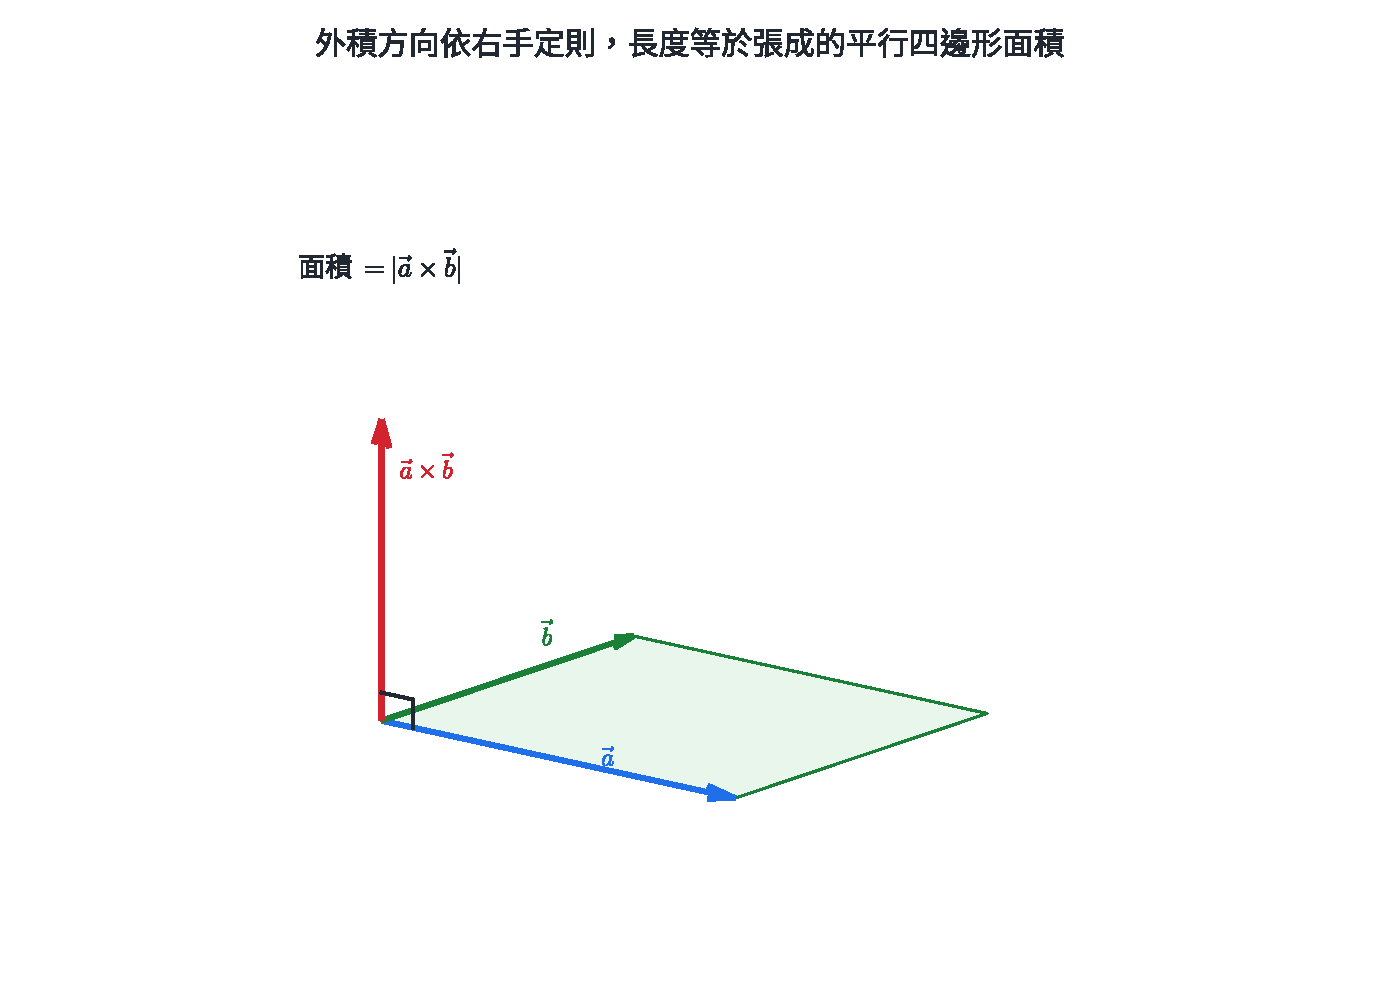
\includegraphics[width=0.84\linewidth,height=\textheight,keepaspectratio,alt={圖 8｜\textbackslash vec a\textbackslash times\textbackslash vec b 垂直兩向量張成的平面，長度等於平行四邊形面積。}]{assets/數A4-1-外積方向與面積.pdf}
\caption{圖 8｜\(\vec a\times\vec b\) 垂直兩向量張成的平面，長度等於平行四邊形面積。}
\end{figure}

若

\[
\vec a=(a_1,a_2,a_3),\qquad
\vec b=(b_1,b_2,b_3),
\]

則坐標公式為

\[
\boxed{
\vec a\times\vec b
=
\bigl(
a_2b_3-a_3b_2,
a_3b_1-a_1b_3,
a_1b_2-a_2b_1
\bigr)
}.
\]

公式可用形式行列式記憶：

\[
\vec a\times\vec b
=
\begin{vmatrix}
\vec i&\vec j&\vec k\\
a_1&a_2&a_3\\
b_1&b_2&b_3
\end{vmatrix}.
\]

沿第一列展開時，\(\vec j\) 項帶負號，因此第二分量寫成 \(a_3b_1-a_1b_3\)。

外積的重要性質為

\[
\vec b\times\vec a=-(\vec a\times\vec b),
\]

\[
(s\vec a+t\vec b)\times\vec c
=s(\vec a\times\vec c)+t(\vec b\times\vec c),
\]

\[
\vec a\times\vec b=\vec0
\iff
\vec a,\vec b\text{ 中有零向量或兩向量平行}.
\]

順序交換會反轉方向，但面積 \(|\vec a\times\vec b|\) 保持不變。

\subsection{4.2 面積、法向量與點線距離}\label{ux9762ux7a4dux6cd5ux5411ux91cfux8207ux9edeux7ddaux8dddux96e2}

由同一點出發的 \(\vec a,\vec b\) 張成：

\[
\boxed{
\text{平行四邊形面積}=|\vec a\times\vec b|
},
\]

\[
\boxed{
\text{三角形面積}=\frac12|\vec a\times\vec b|
}.
\]

\(\vec a\times\vec b\) 同時給出該平面的法向方向。電腦圖學以表面法向判斷哪一面朝向光源；三維掃描與 CAD 也用法向描述曲面朝向。

若直線通過 \(A\)、方向為 \(\vec d\)，點 \(P\) 到直線的距離還可寫成

\[
\boxed{
d(P,L)=\frac{|\overrightarrow{AP}\times\vec d|}{|\vec d|}
}.
\]

因為分子是以 \(|\vec d|\) 為底、點線距離為高的平行四邊形面積。這與上一節的投影公式是同一個幾何量的兩種算法。

\subsection{4.3 三階行列式}\label{ux4e09ux968eux884cux5217ux5f0f}

三個向量 \(\vec a=(a_1,a_2,a_3)\)、\(\vec b=(b_1,b_2,b_3)\)、\(\vec c=(c_1,c_2,c_3)\) 排成三階行列式：

\[
\det(\vec a,\vec b,\vec c)
=
\begin{vmatrix}
a_1&a_2&a_3\\
b_1&b_2&b_3\\
c_1&c_2&c_3
\end{vmatrix}.
\]

沿第一列展開：

\[
\boxed{
\begin{aligned}
\det(\vec a,\vec b,\vec c)
={}&a_1(b_2c_3-b_3c_2)\\
&-a_2(b_1c_3-b_3c_1)\\
&+a_3(b_1c_2-b_2c_1).
\end{aligned}
}
\]

也可用薩魯法則：把前兩欄抄到右側，右下方向的三個乘積相加，右上方向的三個乘積相減。

\begin{figure}
\centering
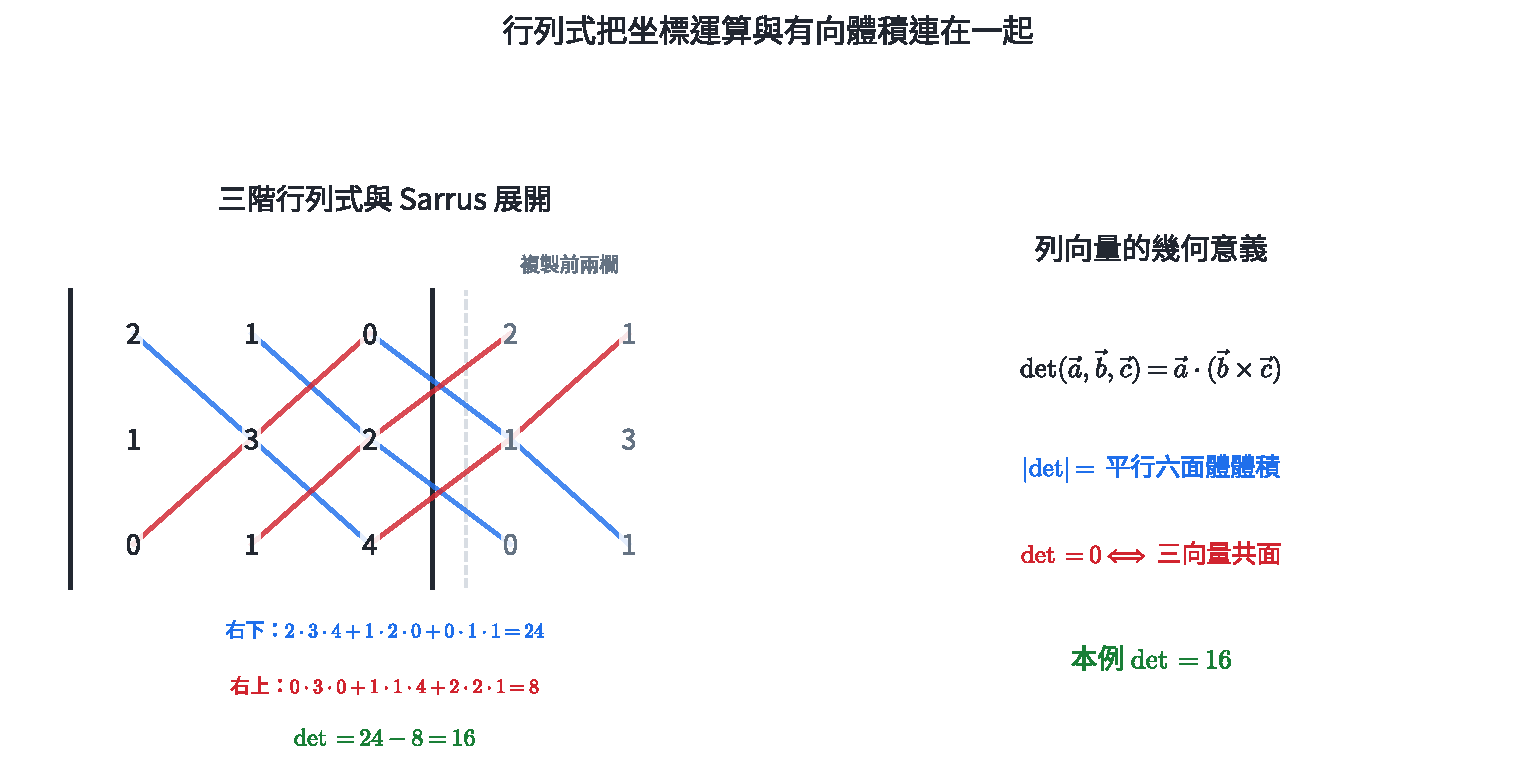
\includegraphics[width=0.92\linewidth,height=\textheight,keepaspectratio,alt={圖 9｜三階行列式的計算與幾何意義。符號保留三個方向的排列順序。}]{assets/數A4-1-三階行列式.pdf}
\caption{圖 9｜三階行列式的計算與幾何意義。符號保留三個方向的排列順序。}
\end{figure}

行列式具有三項對計算很有用的性質：

\begin{enumerate}
\def\labelenumi{\arabic{enumi}.}
\tightlist
\item
  交換任兩列，值變號；
\item
  某一列乘 \(k\)，行列式也乘 \(k\)；
\item
  某一列加上另一列的倍數，值保持不變。
\end{enumerate}

若兩列相同、成比例，或某列是另外兩列的線性組合，行列式為 \(0\)。這些情形都表示三個方向無法張成真正的三維體積。

\subsection{4.4 三重積、體積與共面}\label{ux4e09ux91cdux7a4dux9ad4ux7a4dux8207ux5171ux9762}

先用 \(\vec b\times\vec c\) 建立底面法向與底面積，再與 \(\vec a\) 做內積：

\[
\boxed{
\vec a\cdot(\vec b\times\vec c)
=\det(\vec a,\vec b,\vec c)
}.
\]

其絕對值為三向量張成的平行六面體體積：

\[
\boxed{
V_{\text{平行六面體}}
=|\vec a\cdot(\vec b\times\vec c)|
}.
\]

\begin{figure}
\centering
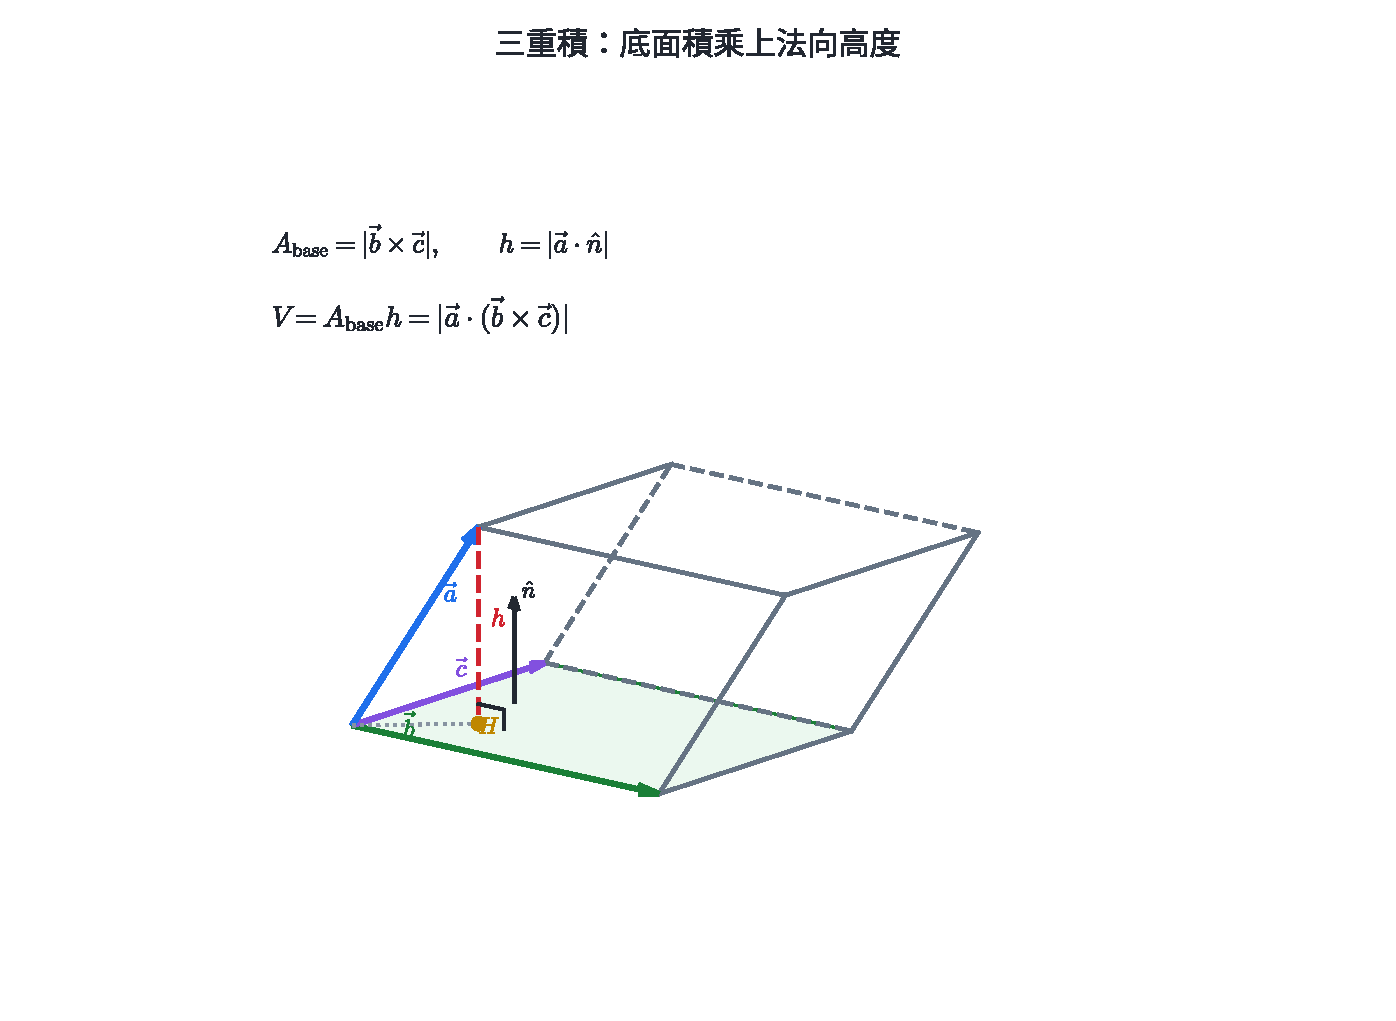
\includegraphics[width=0.84\linewidth,height=\textheight,keepaspectratio,alt={圖 10｜\textbackslash vec b,\textbackslash vec c 張成底面，\textbackslash vec a 在底面法向上的分量給出高，因此體積為 \textbar\textbackslash vec a\textbackslash cdot(\textbackslash vec b\textbackslash times\textbackslash vec c)\textbar。}]{assets/數A4-1-三重積與體積.pdf}
\caption{圖 10｜\(\vec b,\vec c\) 張成底面，\(\vec a\) 在底面法向上的分量給出高，因此體積為 \(|\vec a\cdot(\vec b\times\vec c)|\)。}
\end{figure}

若四面體從同一頂點引出三條棱 \(\vec a,\vec b,\vec c\)，它的體積為相應平行六面體的六分之一：

\[
\boxed{
V_{\text{四面體}}
=\frac16|\vec a\cdot(\vec b\times\vec c)|
}.
\]

三個向量共面的條件為

\[
\boxed{
\vec a,\vec b,\vec c\text{ 共面}
\iff
\det(\vec a,\vec b,\vec c)=0
}.
\]

若考慮四點 \(A,B,C,D\)，以同一基準點 \(A\) 形成 \(\overrightarrow{AB},\overrightarrow{AC},\overrightarrow{AD}\)，再檢查三重積是否為 \(0\)。

\subsection{4.5 外積的直接應用：力矩}\label{ux5916ux7a4dux7684ux76f4ux63a5ux61c9ux7528ux529bux77e9}

一個力造成的轉動效果同時取決於施力大小、施力點到轉軸的距離，以及施力方向。以轉軸上的基準點為起點，令 \(\vec r\) 指向施力點，力矩為

\[
\boxed{
\vec\tau=\vec r\times\vec F
}.
\]

大小為

\[
\boxed{
|\vec\tau|=rF\sin\theta
}.
\]

\begin{figure}
\centering
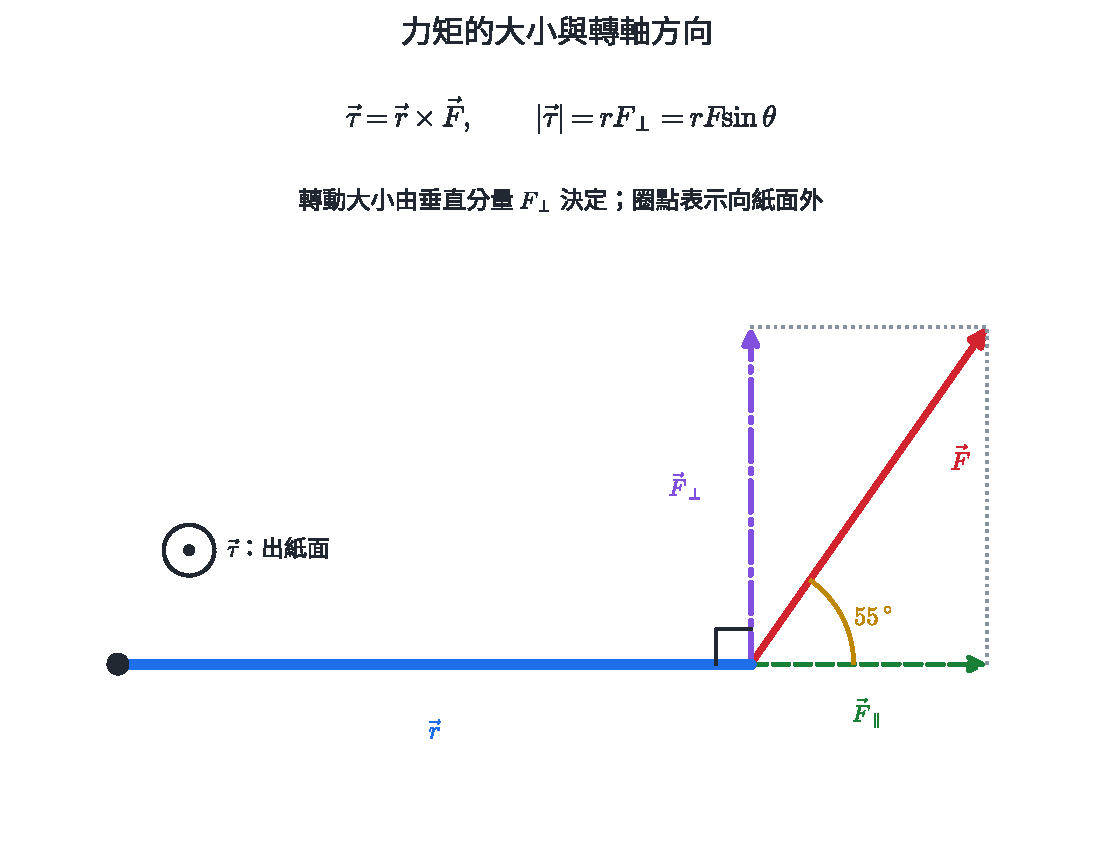
\includegraphics[width=0.88\linewidth,height=\textheight,keepaspectratio,alt={圖 11｜力矩只取施力中垂直槓桿的分量；方向由右手定則決定轉軸方向。}]{assets/數A4-1-力矩模型.pdf}
\caption{圖 11｜力矩只取施力中垂直槓桿的分量；方向由右手定則決定轉軸方向。}
\end{figure}

門把設在遠離鉸鏈處，是為了放大 \(r\)；扳手與螺帽的連線接近垂直施力，是為了使 \(\sin\theta\) 接近 \(1\)。這兩項設計都直接來自外積長度。

\begin{HandoutWorkedExample}

\subsection{完整示範｜外積、法向量與三角形面積}\label{ux5b8cux6574ux793aux7bc4ux5916ux7a4dux6cd5ux5411ux91cfux8207ux4e09ux89d2ux5f62ux9762ux7a4d}

設

\[
A=(1,0,1),\quad B=(3,1,2),\quad C=(2,4,0).
\]

取同一起點 \(A\)：

\[
\overrightarrow{AB}=(2,1,1),\qquad
\overrightarrow{AC}=(1,4,-1).
\]

計算外積：

\[
\overrightarrow{AB}\times\overrightarrow{AC}
=
\begin{vmatrix}
\vec i&\vec j&\vec k\\
2&1&1\\
1&4&-1
\end{vmatrix}
=(-5,3,7).
\]

核對法向性：

\[
(-5,3,7)\cdot(2,1,1)=-10+3+7=0,
\]

\[
(-5,3,7)\cdot(1,4,-1)=-5+12-7=0.
\]

所以 \((-5,3,7)\) 是平面 \(ABC\) 的一個法向量。三角形面積為

\[
[ABC]
=\frac12\sqrt{25+9+49}
=\boxed{\frac{\sqrt{83}}2}.
\]

\end{HandoutWorkedExample}

\begin{HandoutWorkedExample}

\subsection{完整示範｜用外積求點到直線的距離}\label{ux5b8cux6574ux793aux7bc4ux7528ux5916ux7a4dux6c42ux9edeux5230ux76f4ux7ddaux7684ux8dddux96e2}

直線通過 \(A=(1,1,0)\)，方向向量為 \(\vec d=(2,-1,2)\)；點 \(P=(3,2,4)\)。求點線距離。

\[
\overrightarrow{AP}=(2,1,4).
\]

\[
\overrightarrow{AP}\times\vec d
=
\begin{vmatrix}
\vec i&\vec j&\vec k\\
2&1&4\\
2&-1&2
\end{vmatrix}
=(6,4,-4).
\]

所以

\[
d(P,L)
=\frac{\sqrt{6^2+4^2+(-4)^2}}{\sqrt{2^2+(-1)^2+2^2}}
=\frac{\sqrt{68}}3
=\boxed{\frac{2\sqrt{17}}3}.
\]

分子是以方向向量為底的平行四邊形面積，除以底長後得到高。

\end{HandoutWorkedExample}

\begin{HandoutWorkedExample}

\subsection{完整示範｜行列式的列運算}\label{ux5b8cux6574ux793aux7bc4ux884cux5217ux5f0fux7684ux5217ux904bux7b97}

計算

\[
D=
\begin{vmatrix}
1&2&3\\
2&5&8\\
1&0&1
\end{vmatrix}.
\]

先做保持行列式值的列運算：第二列減去第一列的 \(2\) 倍，第三列減去第一列：

\[
D=
\begin{vmatrix}
1&2&3\\
0&1&2\\
0&-2&-2
\end{vmatrix}.
\]

再把第三列加上第二列的 \(2\) 倍：

\[
D=
\begin{vmatrix}
1&2&3\\
0&1&2\\
0&0&2
\end{vmatrix}=1\cdot1\cdot2=\boxed2.
\]

上三角形式的行列式等於對角線乘積。

\end{HandoutWorkedExample}

\begin{HandoutWorkedExample}

\subsection{完整示範｜四面體體積與共面參數}\label{ux5b8cux6574ux793aux7bc4ux56dbux9762ux9ad4ux9ad4ux7a4dux8207ux5171ux9762ux53c3ux6578}

設

\[
A=(0,0,0),\quad B=(2,0,0),\quad C=(0,3,0),\quad D=(1,1,k).
\]

從 \(A\) 引出三向量：

\[
\overrightarrow{AB}=(2,0,0),\quad
\overrightarrow{AC}=(0,3,0),\quad
\overrightarrow{AD}=(1,1,k).
\]

三重積為

\[
\det
\begin{pmatrix}
2&0&0\\
0&3&0\\
1&1&k
\end{pmatrix}
=6k.
\]

四面體體積為

\[
V=\frac16|6k|=\boxed{|k|}.
\]

四點共面恰好對應體積為 \(0\)，所以

\[
\boxed{k=0}.
\]

這也符合坐標圖像：前三點都在 \(xy\) 平面，\(D\) 的 \(z\) 坐標為 \(0\) 時也落在同一平面。

\end{HandoutWorkedExample}

\begin{HandoutWorkedExample}

\subsection{完整示範｜施力方向如何影響力矩}\label{ux5b8cux6574ux793aux7bc4ux65bdux529bux65b9ux5411ux5982ux4f55ux5f71ux97ffux529bux77e9}

長 \(0.40\ \mathrm{m}\) 的扳手受到 \(50\ \mathrm{N}\) 的力，力與扳手夾角為 \(60^\circ\)。求力矩大小；再比較同樣大小的力以 \(30^\circ\) 施加時的力矩。

第一種施力：

\[
\tau_1=rF\sin60^\circ
=0.40(50)\frac{\sqrt3}{2}
=10\sqrt3\ \mathrm{N\,m}
\approx17.3\ \mathrm{N\,m}.
\]

第二種施力：

\[
\tau_2=rF\sin30^\circ
=0.40(50)\frac12
=10\ \mathrm{N\,m}.
\]

扳手長度與力的大小相同時，垂直分力較大的 \(60^\circ\) 施力產生較大力矩。

\end{HandoutWorkedExample}

\begin{HandoutSelfCheck}

\subsection{節末練習｜外積、面積與體積}\label{ux7bc0ux672bux7df4ux7fd2ux5916ux7a4dux9762ux7a4dux8207ux9ad4ux7a4d}

\begin{enumerate}
\def\labelenumi{\arabic{enumi}.}
\tightlist
\item
  計算 \((1,2,3)\times(2,-1,1)\)，並以內積核對所得向量垂直於原兩向量。
\item
  \(A=(0,0,0)\)、\(B=(2,1,0)\)、\(C=(1,3,2)\)。求三角形 \(ABC\) 面積與一個法向量。
\item
  直線通過 \(A=(1,0,1)\)、方向為 \((1,2,2)\)，求點 \(P=(3,1,4)\) 到直線的距離。
\item
  計算 \(\begin{vmatrix}2&1&0\\1&3&2\\0&1&4\end{vmatrix}\)。
\item
  判斷 \(\vec a=(1,0,2)\)、\(\vec b=(0,2,1)\)、\(\vec c=(2,2,5)\) 是否共面。
\item
  四面體 \(OABC\) 中，\(A=(2,0,0)\)、\(B=(0,3,0)\)、\(C=(1,1,4)\)。求體積。若把 \(C\) 改成 \((1,1,h)\)，體積為 \(6\)，求 \(h\)。
\end{enumerate}

\textbf{解答}

\begin{enumerate}
\def\labelenumi{\arabic{enumi}.}
\tightlist
\item
  外積為 \((5,5,-5)\)。與第一向量內積 \(5+10-15=0\)；與第二向量內積 \(10-5-5=0\)。
\item
  \(\overrightarrow{AB}=(2,1,0)\)、\(\overrightarrow{AC}=(1,3,2)\)，外積為 \((2,-4,5)\)。法向量可取 \((2,-4,5)\)；面積為 \(\sqrt{4+16+25}/2=3\sqrt5/2\)。
\item
  \(\overrightarrow{AP}=(2,1,3)\)，與方向向量的外積為 \((-4,-1,3)\)。距離為 \(\sqrt{26}/3\)。
\item
  沿第一列展開：\(2(12-2)-1(4-0)=16\)。
\item
  \(\vec c=2\vec a+\vec b\)，因此共面；等價地，\(\det(\vec a,\vec b,\vec c)=0\)。
\item
  三重積為 \(2\cdot3\cdot4=24\)，體積為 \(24/6=4\)。改為 \(h\) 時體積為 \(|6h|/6=|h|\)，故 \(h=6\) 或 \(h=-6\)。
\end{enumerate}

\end{HandoutSelfCheck}

\section{5. 核心整理}\label{ux6838ux5fc3ux6574ux7406}

\subsection{位置與坐標}\label{ux4f4dux7f6eux8207ux5750ux6a19}

\[
\overrightarrow{AB}=B-A,
\qquad
AB=|B-A|,
\qquad
P_{AP:PB=m:n}=\frac{nA+mB}{m+n}.
\]

兩直線沒有交點時，再用共平面條件區分平行與歪斜。直線垂直平面，可由它垂直平面內兩條相交直線判定。

\subsection{內積與投影}\label{ux5167ux7a4dux8207ux6295ux5f71}

\[
\vec a\cdot\vec b
=a_1b_1+a_2b_2+a_3b_3
=|\vec a|\,|\vec b|\cos\theta.
\]

\[
\operatorname{proj}_{\vec b}\vec a
=\frac{\vec a\cdot\vec b}{|\vec b|^2}\vec b,
\qquad
|\vec a\cdot\vec b|\le|\vec a|\,|\vec b|.
\]

\subsection{外積與三重積}\label{ux5916ux7a4dux8207ux4e09ux91cdux7a4d}

\[
\vec a\times\vec b
=
(a_2b_3-a_3b_2,
a_3b_1-a_1b_3,
a_1b_2-a_2b_1).
\]

\[
[\triangle]=\frac12|\vec a\times\vec b|,
\qquad
V_{\text{平行六面體}}
=|\vec a\cdot(\vec b\times\vec c)|,
\]

\[
V_{\text{四面體}}
=\frac16|\vec a\cdot(\vec b\times\vec c)|.
\]

內積保留沿指定方向的分量；外積建立垂直方向與面積；三重積再取第三方向的高度，得到體積。

\section{6. 分層題與跨節整合題}\label{ux5206ux5c64ux984cux8207ux8de8ux7bc0ux6574ux5408ux984c}

\subsection{題目 1｜坐標平面、距離與對稱}\label{ux984cux76ee-1ux5750ux6a19ux5e73ux9762ux8dddux96e2ux8207ux5c0dux7a31}

點 \(P=(-2,6,3)\)。

\begin{enumerate}
\def\labelenumi{\arabic{enumi}.}
\tightlist
\item
  求 \(P\) 在 \(yz\) 平面上的投影；
\item
  求 \(P\) 到 \(x\) 軸的距離；
\item
  求 \(P\) 關於 \(zx\) 平面的對稱點。
\end{enumerate}

\subsection{題目 2｜位移、長度與分點}\label{ux984cux76ee-2ux4f4dux79fbux9577ux5ea6ux8207ux5206ux9ede}

\(A=(-1,2,1)\)、\(B=(3,-2,5)\)。求 \(\overrightarrow{AB}\)、\(AB\)，以及由 \(A\) 向 \(B\) 前進全程四分之一時的位置 \(P\)。

\subsection{題目 3｜空間位置關係}\label{ux984cux76ee-3ux7a7aux9593ux4f4dux7f6eux95dcux4fc2}

正方體 \(ABCD-EFGH\) 中，\(E,F,G,H\) 分別在 \(A,B,C,D\) 正上方。

\begin{enumerate}
\def\labelenumi{\arabic{enumi}.}
\tightlist
\item
  判斷 \(AB\) 與 \(CG\) 的位置關係；
\item
  判斷 \(AC\) 與 \(EG\) 的位置關係；
\item
  說明 \(AE\) 與平面 \(ABCD\) 的關係。
\end{enumerate}

\subsection{題目 4｜直線與平面的夾角}\label{ux984cux76ee-4ux76f4ux7ddaux8207ux5e73ux9762ux7684ux593eux89d2}

點 \(P\) 到平面 \(E\) 的垂足為 \(A\)。\(B\) 在 \(E\) 上，\(PA=12\)、\(AB=5\)。求 \(PB\) 長，以及 \(PB\) 與平面 \(E\) 的夾角。

\subsection{題目 5｜三維線性組合}\label{ux984cux76ee-5ux4e09ux7dadux7ddaux6027ux7d44ux5408}

設

\[
\vec a=(1,1,0),\qquad
\vec b=(1,0,1),\qquad
\vec c=(0,1,1).
\]

求 \(x,y,z\) 使 \(x\vec a+y\vec b+z\vec c=(7,5,6)\)。

\subsection{題目 6｜內積與夾角}\label{ux984cux76ee-6ux5167ux7a4dux8207ux593eux89d2}

設 \(\vec a=(1,2,2)\)、\(\vec b=(2,2,1)\)。求兩向量夾角，並判斷它是銳角、直角或鈍角。

\subsection{題目 7｜正射影與垂直分解}\label{ux984cux76ee-7ux6b63ux5c04ux5f71ux8207ux5782ux76f4ux5206ux89e3}

把 \(\vec a=(4,2,-1)\) 分解成平行與垂直於 \(\vec b=(1,2,2)\) 的兩部分，並求垂直分量的長度。

\subsection{題目 8｜柯西不等式與極值位置}\label{ux984cux76ee-8ux67efux897fux4e0dux7b49ux5f0fux8207ux6975ux503cux4f4dux7f6e}

已知 \(x^2+y^2+z^2=16\)，求 \(x-2y+2z\) 的最大值、最小值，以及各自的等號位置。

\subsection{題目 9｜外積與面積}\label{ux984cux76ee-9ux5916ux7a4dux8207ux9762ux7a4d}

設 \(\vec a=(2,1,0)\)、\(\vec b=(1,0,3)\)。求 \(\vec a\times\vec b\)，以及兩向量張成的三角形面積。

\subsection{題目 10｜點到直線的距離}\label{ux984cux76ee-10ux9edeux5230ux76f4ux7ddaux7684ux8dddux96e2}

直線 \(L\) 通過 \(A=(0,1,0)\)，方向向量為 \(\vec d=(2,1,-2)\)。求點 \(P=(1,3,4)\) 到 \(L\) 的距離。

\subsection{題目 11｜三階行列式}\label{ux984cux76ee-11ux4e09ux968eux884cux5217ux5f0f}

用展開或列運算計算

\[
\begin{vmatrix}
1&2&0\\
0&1&3\\
2&-1&1
\end{vmatrix}.
\]

\subsection{題目 12｜四面體體積}\label{ux984cux76ee-12ux56dbux9762ux9ad4ux9ad4ux7a4d}

四面體 \(OABC\) 中，

\[
O=(0,0,0),\quad A=(1,0,1),\quad B=(0,2,1),\quad C=(3,1,0).
\]

求四面體體積。

\subsection{題目 13｜跨節整合：投影三角形與三垂線}\label{ux984cux76ee-13ux8de8ux7bc0ux6574ux5408ux6295ux5f71ux4e09ux89d2ux5f62ux8207ux4e09ux5782ux7dda}

平面 \(E\) 為 \(xy\) 平面，\(A=(0,0,0)\)、\(P=(0,0,6)\)、\(B=(8,0,0)\)、\(C=(8,5,0)\)。

\begin{enumerate}
\def\labelenumi{\arabic{enumi}.}
\tightlist
\item
  說明 \(A\) 是 \(P\) 在 \(E\) 上的垂足；
\item
  求 \(PB\) 與平面 \(E\) 的夾角；
\item
  用三垂線定理與內積各證明一次 \(PB\perp BC\)。
\end{enumerate}

\subsection{題目 14｜跨節整合：動點三角形的最小面積}\label{ux984cux76ee-14ux8de8ux7bc0ux6574ux5408ux52d5ux9edeux4e09ux89d2ux5f62ux7684ux6700ux5c0fux9762ux7a4d}

\(A=(1,0,0)\)、\(B=(3,1,1)\)、\(C=(1,t,2)\)。求三角形 \(ABC\) 面積的最小值，以及此時的 \(t\)。

\subsection{題目 15｜跨節整合：共面參數與四面體體積}\label{ux984cux76ee-15ux8de8ux7bc0ux6574ux5408ux5171ux9762ux53c3ux6578ux8207ux56dbux9762ux9ad4ux9ad4ux7a4d}

設

\[
A=(1,0,0),\quad B=(0,1,0),\quad C=(0,0,1),\quad D=(t,t,t).
\]

\begin{enumerate}
\def\labelenumi{\arabic{enumi}.}
\tightlist
\item
  求四點共面時的 \(t\)；
\item
  求四面體 \(ABCD\) 的體積關於 \(t\) 的公式；
\item
  若體積為 \(1/3\)，求 \(t\)。
\end{enumerate}

\subsection{題目 16｜跨節整合：力的投影、做功與力矩}\label{ux984cux76ee-16ux8de8ux7bc0ux6574ux5408ux529bux7684ux6295ux5f71ux505aux529fux8207ux529bux77e9}

以鉸鏈為原點，門把位置向量為

\[
\vec r=(0.40,0,0)\ \mathrm{m},
\]

施力為

\[
\vec F=(30,40,0)\ \mathrm{N}.
\]

\begin{enumerate}
\def\labelenumi{\arabic{enumi}.}
\tightlist
\item
  把 \(\vec F\) 分解成平行與垂直於 \(\vec r\) 的部分；
\item
  求力矩向量 \(\vec\tau=\vec r\times\vec F\)；
\item
  若作用點沿 \(\vec s=(2,1,0)\ \mathrm{m}\) 位移，求此力所做的功 \(W=\vec F\cdot\vec s\)；
\item
  說明內積與外積在本題各自保留哪個方向的效果。
\end{enumerate}

\section{7. 分層題與跨節整合題詳解}\label{ux5206ux5c64ux984cux8207ux8de8ux7bc0ux6574ux5408ux984cux8a73ux89e3}

\subsection{第 1 題}\label{ux7b2c-1-ux984c}

\(yz\) 平面的方程是 \(x=0\)，投影保留 \(y,z\) 分量，所以

\[
P_{yz}=(0,6,3).
\]

到 \(x\) 軸的距離由垂直於 \(x\) 軸的 \(y,z\) 分量決定：

\[
d(P,x\text{ 軸})
=\sqrt{6^2+3^2}
=3\sqrt5.
\]

\(zx\) 平面的方程是 \(y=0\)。關於它鏡射時，\(x,z\) 保持、\(y\) 反號，所以對稱點為

\[
\boxed{(-2,-6,3)}.
\]

\subsection{第 2 題}\label{ux7b2c-2-ux984c}

點相減得到位移：

\[
\overrightarrow{AB}=B-A=(4,-4,4).
\]

因此

\[
AB=\sqrt{4^2+(-4)^2+4^2}=4\sqrt3.
\]

由 \(A\) 前進全程四分之一：

\[
P=A+\frac14\overrightarrow{AB}
=(-1,2,1)+(1,-1,1)
=\boxed{(0,1,2)}.
\]

核對 \(P-A=(1,-1,1)\)，確為 \(B-A\) 的四分之一。

\subsection{第 3 題}\label{ux7b2c-3-ux984c}

\begin{enumerate}
\def\labelenumi{\arabic{enumi}.}
\item
  \(AB\) 是底面棱，\(CG\) 是鉛直棱。兩線沒有交點、方向不平行，且無共同平面，所以是歪斜線。
\item
  \(AC\) 是底面對角線，\(EG\) 是頂面對應對角線；兩線方向相同，且共同位於斜截面 \(ACEG\)，所以平行。
\item
  \(AE\) 同時垂直底面內相交的 \(AB\) 與 \(AD\)，因此

  \[
  \boxed{AE\perp\text{平面 }ABCD}.
  \]
\end{enumerate}

判斷歪斜時使用了「無交點、方向不平行、不共平面」三項資訊。

\subsection{第 4 題}\label{ux7b2c-4-ux984c}

\(PA\perp E\)，所以 \(PA\perp AB\)。在直角三角形 \(PAB\) 中，

\[
PB=\sqrt{12^2+5^2}=13.
\]

\(PB\) 在平面上的投影是 \(AB\)。設 \(PB\) 與平面夾角為 \(\theta=\angle PBA\)，則

\[
\sin\theta=\frac{PA}{PB}=\frac{12}{13}.
\]

所以

\[
\boxed{\theta=\sin^{-1}\!\left(\frac{12}{13}\right)\approx67.4^\circ}.
\]

\subsection{第 5 題}\label{ux7b2c-5-ux984c}

比較 \(x\vec a+y\vec b+z\vec c=(7,5,6)\) 的三個分量：

\[
\begin{cases}
x+y=7,\\
x+z=5,\\
y+z=6.
\end{cases}
\]

前兩式相加再減第三式：

\[
2x=7+5-6=6,
\]

所以 \(x=3\)。再代入得 \(y=4\)、\(z=2\)。因此

\[
\boxed{(7,5,6)=3\vec a+4\vec b+2\vec c}.
\]

\subsection{第 6 題}\label{ux7b2c-6-ux984c}

先算內積與長度：

\[
\vec a\cdot\vec b=2+4+2=8,
\]

\[
|\vec a|=|\vec b|=\sqrt{1+4+4}=3.
\]

因此

\[
\cos\theta=\frac89,
\qquad
\boxed{\theta=\cos^{-1}\!\left(\frac89\right)\approx27.3^\circ}.
\]

內積為正，所以角為銳角；數值結果也符合。

\subsection{第 7 題}\label{ux7b2c-7-ux984c}

\[
\vec a\cdot\vec b=4+4-2=6,
\qquad
|\vec b|^2=1+4+4=9.
\]

平行分量為

\[
\vec a_\parallel
=\frac69\vec b
=\left(\frac23,\frac43,\frac43\right).
\]

垂直分量為

\[
\vec a_\perp
=\vec a-\vec a_\parallel
=\left(\frac{10}3,\frac23,-\frac73\right).
\]

核對：

\[
\vec a_\perp\cdot\vec b
=\frac{10}3+\frac43-\frac{14}3=0.
\]

其長度為

\[
|\vec a_\perp|
=\frac13\sqrt{100+4+49}
=\boxed{\sqrt{17}}.
\]

\subsection{第 8 題}\label{ux7b2c-8-ux984c}

把目標式看成 \((x,y,z)\) 與 \((1,-2,2)\) 的內積。由柯西不等式，

\[
|x-2y+2z|
\le\sqrt{x^2+y^2+z^2}\sqrt{1+4+4}
=4\cdot3=12.
\]

所以最大值為 \(12\)，最小值為 \(-12\)。

最大值時，\((x,y,z)\) 與 \((1,-2,2)\) 同方向，且長度為 \(4\)：

\[
(x,y,z)=\frac43(1,-2,2)
=\left(\frac43,-\frac83,\frac83\right).
\]

最小值的位置是其反向：

\[
\boxed{\left(-\frac43,\frac83,-\frac83\right)}.
\]

\subsection{第 9 題}\label{ux7b2c-9-ux984c}

\[
\vec a\times\vec b
=
\begin{vmatrix}
\vec i&\vec j&\vec k\\
2&1&0\\
1&0&3
\end{vmatrix}
=(3,-6,-1).
\]

核對 \((3,-6,-1)\cdot(2,1,0)=0\)、\((3,-6,-1)\cdot(1,0,3)=0\)。

平行四邊形面積為 \(\sqrt{9+36+1}=\sqrt{46}\)，所以三角形面積為

\[
\boxed{\frac{\sqrt{46}}2}.
\]

\subsection{第 10 題}\label{ux7b2c-10-ux984c}

\[
\overrightarrow{AP}=P-A=(1,2,4).
\]

\[
\overrightarrow{AP}\times\vec d
=
\begin{vmatrix}
\vec i&\vec j&\vec k\\
1&2&4\\
2&1&-2
\end{vmatrix}
=(-8,10,-3).
\]

因此

\[
d(P,L)
=\frac{\sqrt{64+100+9}}{\sqrt{4+1+4}}
=\boxed{\frac{\sqrt{173}}3}.
\]

\subsection{第 11 題}\label{ux7b2c-11-ux984c}

沿第一列展開：

\[
\begin{aligned}
D
&=1
\begin{vmatrix}1&3\\-1&1\end{vmatrix}
-2
\begin{vmatrix}0&3\\2&1\end{vmatrix}\\
&=(1+3)-2(0-6)\\
&=4+12\\
&=\boxed{16}.
\end{aligned}
\]

也可把第三列減去第一列的 \(2\) 倍，再沿第一欄展開，會得到相同結果。

\subsection{第 12 題}\label{ux7b2c-12-ux984c}

由原點出發的三條棱為

\[
\overrightarrow{OA}=(1,0,1),\quad
\overrightarrow{OB}=(0,2,1),\quad
\overrightarrow{OC}=(3,1,0).
\]

先算

\[
\overrightarrow{OB}\times\overrightarrow{OC}
=(-1,3,-6).
\]

三重積為

\[
\overrightarrow{OA}\cdot
(\overrightarrow{OB}\times\overrightarrow{OC})
=-1-6=-7.
\]

體積取絕對值並除以 \(6\)：

\[
\boxed{V=\frac{|{-7}|}{6}=\frac76}.
\]

\subsection{第 13 題}\label{ux7b2c-13-ux984c}

平面 \(E\) 是 \(z=0\)。\(A=(0,0,0)\) 與 \(P=(0,0,6)\) 只差 \(z\) 分量，所以 \(A\) 是 \(P\) 在 \(E\) 上的投影，而且 \(PA\) 的方向 \((0,0,1)\) 垂直平面內的 \(x,y\) 方向。

\(PB\) 在 \(E\) 上的投影是 \(AB\)。\(PA=6\)、\(AB=8\)，因此 \(PB=10\)。設夾角為 \(\theta\)：

\[
\sin\theta=\frac6{10}=\frac35,
\qquad
\boxed{\theta\approx36.9^\circ}.
\]

接著

\[
\overrightarrow{AB}=(8,0,0),
\qquad
\overrightarrow{BC}=(0,5,0),
\]

所以 \(AB\perp BC\)。\(AB\) 是 \(PB\) 的平面投影，由三垂線定理得 \(PB\perp BC\)。

用內積直接核對：

\[
\overrightarrow{BP}=P-B=(-8,0,6),
\]

\[
\overrightarrow{BP}\cdot\overrightarrow{BC}
=(-8,0,6)\cdot(0,5,0)=0.
\]

兩種證明都把斜線分解成水平投影與鉛直高度。

\subsection{第 14 題}\label{ux7b2c-14-ux984c}

從 \(A\) 引出兩邊：

\[
\overrightarrow{AB}=(2,1,1),
\qquad
\overrightarrow{AC}=(0,t,2).
\]

外積為

\[
\overrightarrow{AB}\times\overrightarrow{AC}
=(2-t,-4,2t).
\]

所以三角形面積平方為

\[
[ABC]^2
=\frac14\left[(2-t)^2+16+4t^2\right]
=\frac14(5t^2-4t+20).
\]

配方：

\[
5t^2-4t+20
=5\left(t-\frac25\right)^2+\frac{96}{5}.
\]

因此 \(t=2/5\) 時面積最小，最小值為

\[
\boxed{
[ABC]_{\min}
=\frac12\sqrt{\frac{96}{5}}
=\frac{2\sqrt{30}}5
}.
\]

\subsection{第 15 題}\label{ux7b2c-15-ux984c}

以 \(A\) 為共同起點：

\[
\overrightarrow{AB}=(-1,1,0),
\]

\[
\overrightarrow{AC}=(-1,0,1),
\]

\[
\overrightarrow{AD}=(t-1,t,t).
\]

先算

\[
\overrightarrow{AB}\times\overrightarrow{AC}=(1,1,1).
\]

三重積為

\[
(\overrightarrow{AB}\times\overrightarrow{AC})
\cdot\overrightarrow{AD}
=(t-1)+t+t=3t-1.
\]

四點共面時三重積為 \(0\)，所以

\[
\boxed{t=\frac13}.
\]

四面體體積為

\[
\boxed{V(t)=\frac{|3t-1|}{6}}.
\]

若 \(V=1/3\)，則

\[
\frac{|3t-1|}{6}=\frac13
\quad\Longrightarrow\quad
|3t-1|=2.
\]

故

\[
3t-1=2\quad\text{或}\quad3t-1=-2,
\]

\[
\boxed{t=1\quad\text{或}\quad t=-\frac13}.
\]

\subsection{第 16 題}\label{ux7b2c-16-ux984c}

\(\vec r\) 沿 \(x\) 軸，所以 \(\vec F\) 平行於 \(\vec r\) 的部分保留 \(x\) 分量：

\[
\vec F_\parallel=(30,0,0)\ \mathrm N,
\]

垂直部分為

\[
\vec F_\perp=(0,40,0)\ \mathrm N.
\]

力矩向量為

\[
\vec\tau
=\vec r\times\vec F
=(0.40,0,0)\times(30,40,0)
=\boxed{(0,0,16)\ \mathrm{N\,m}}.
\]

平行分力與 \(\vec r\) 的外積為零；垂直分力完整貢獻力矩。

做功為力與位移的內積：

\[
W=\vec F\cdot\vec s
=(30,40,0)\cdot(2,1,0)
=60+40
=\boxed{100\ \mathrm J}.
\]

本題中，內積保留力沿位移方向的有效分量，用來計算能量轉移；外積保留力垂直於位置向量的有效分量，用來計算轉動效果。兩種乘法各自回答不同的方向問題。


\end{document}
